\documentclass[IEEE JOURNAL OF BIOMEDICAL AND HEALTH INFORMATICS]{IEEEtran}
%
% If IEEEtran.cls has not been installed into the LaTeX system files,
% manually specify the path to it like:
%\documentclass[journal]{../sty/IEEEtran}
\usepackage{graphicx}
%\usepackage{subfigure}
\usepackage[misc]{ifsym}
%\usepackage{mathptmx}      % use Times fonts if available on your TeX system

%???????
\usepackage{fontspec}
\setmainfont{Times New Roman}
\usepackage{amsmath}
\usepackage{amssymb}
%\usepackage{mathspec}

\usepackage{algorithm}  
\usepackage{algpseudocode}  
\usepackage{amsmath}  
\renewcommand{\algorithmicrequire}{\textbf{Input:}}  % Use Input in the format of Algorithm  
\renewcommand{\algorithmicensure}{\textbf{Output:}} % Use Output in the format of Algorithm  

\usepackage[numbers,sort&compress]{natbib}
% insert here the call for the packages your document requires
\usepackage{epstopdf}
\usepackage{latexsym}
\usepackage{enumerate}
\usepackage{extarrows}
\usepackage{color}
\usepackage{url}
%\usepackage{mathrsfs}
\usepackage{arydshln}
\usepackage[switch]{lineno}
\usepackage{textcomp}
\usepackage{caption}
\usepackage{subcaption}
\usepackage[labelformat=simple]{subcaption}
\renewcommand\thesubfigure{(\alph{subfigure})}
\usepackage{graphicx}
\usepackage[misc]{ifsym}
%\usepackage{mathptmx}      % use Times fonts if available on your TeX system
%\usepackage{amsmath,amssymb}

% insert here the call for the packages your document requires
\usepackage{epstopdf}
\usepackage{latexsym}
\usepackage{enumerate}
\usepackage{extarrows}
\usepackage{color}
\usepackage{url}
%\usepackage{mathrsfs}
\usepackage{arydshln}
\usepackage{multirow}
\usepackage{subcaption}
\usepackage[switch]{lineno}
%\usepackage{dutchcal} %1?15???
\usepackage{boondox-calo}
\usepackage{amssymb}
\newtheorem{prf}{Proof}
\newtheorem{dfn}{Definition}
\newtheorem{asmpt}{Assumption}
\newtheorem{theorem}{Theorem}
\newcommand{\tabincell}[2]{\begin{tabular}{@{}#1@{}}#2\end{tabular}}
% *** GRAPHICS RELATED PACKAGES ***
%
%\ifCLASSINFOpdf
  % \usepackage[pdftex]{graphicx}
  % declare the path(s) where your graphic files are
  % \graphicspath{{../pdf/}{../jpeg/}}
  % and their extensions so you won't have to specify these with
  % every instance of \includegraphics
  % \DeclareGraphicsExtensions{.pdf,.jpeg,.png}
%\else

%\fi
\hyphenation{op-tical net-works semi-conduc-tor}
\usepackage{xcolor}%???????
\usepackage{colortbl,booktabs}%?????????*rule
\usepackage{color}
\setlength{\textfloatsep}{3pt}
\begin{document}
%\captionsetup{font={small}}
%
% paper title
% can use linebreaks \\ within to get better formatting as desired
% Do not put math or special symbols in the title.

%\linenumbers
\title{Safer and lighter: New Privacy-Preserving joint  Computations for Optimal Location Selection}
%\thanks{S. Liu is with the School of Computer Science and Engineering, Hunan University of Science and Technology, Xiangtan, 411201, China (e-mail: liushanpeng123@outlook.com).}
%\thanks{F. Wu is with the Department of Computer Science and Engineering, Xiamen Institute of Technology, Xiamen 361021, China (e-mail: conjurer1981@gmail.com).}
%\thanks{S. Kumari is with the Department of Mathematics, Ch. Charan Singh University, Meerut, 250005, India (e-mail: saryusiirohi@gmail.com).}
%\thanks{J. J.P.C. Rodrigues is with the National Institute of Telecommunications (Inatel), Santa Rita do Sapuca\'i, MG, Brazil; and with Instituto de Telecomunica\c{c}\~oes, Portugal;  University of Fortaleza (UNIFOR), Fortaleza, CE, Brazil (e-mail: joeljr@ieee.org).}}


%\fi
% note the % following the last \IEEEmembership and also \thanks -
% these prevent an unwanted space from occurring between the last author name
% and the end of the author line. i.e., if you had this:
%
% \author{....lastname \thanks{...} \thanks{...} }
%                     ^------------^------------^----Do not want these spaces!
%
% a space would be appended to the last name and could cause every name on that
% line to be shifted left slightly. This is one of those "LaTeX things". For
% instance, "\textbf{A} \textbf{B}" will typeset as "A B" not "AB". To get
% "AB" then you have to do: "\textbf{A}\textbf{B}"
% \thanks is no different in this regard, so shield the last } of each \thanks
% that ends a line with a % and do not let a space in before the next \thanks.
% Spaces after \IEEEmembership other than the last one are OK (and needed) as
% you are supposed to have spaces between the names. For what it is worth,
% this is a minor point as most people would not even notice if the said evil
% space somehow managed to creep in.



% The paper headers
%\markboth{Journal of \LaTeX\ Class Files,~Vol.~11, No.~4, December~2012}%
%{Shell \MakeLowercase{\textit{et al.}}: Bare Demo of IEEEtran.cls for Journals}


% The only time the second header will appear is for the odd numbered pages
% after the title page when using the twoside option.
%
% *** Note that you probably will NOT want to include the author's ***
% *** name in the headers of peer review papers.                   ***
% You can use \ifCLASSOPTIONpeerreview for conditional compilation here if
% you desire.




% If you want to put a publisher's ID mark on the page you can do it like
% this:
%\IEEEpubid{0000--0000/00\$00.00~\copyright~2012 IEEE}
% Remember, if you use this you must call \IEEEpubidadjcol in the second
% column for its text to clear the IEEEpubid mark.


%\linenumbers
% use for special paper notices
%\IEEEspecialpapernotice{(Invited Paper)}

% make the title area
\maketitle

\begin{abstract}
Edge-supported industrial Internet of Things (IIoT) has recently received significant attention since the edge computing can greatly improve the service quality of IIoT applications. However, edge servers are not fully trusted and are often deployed at the edge of the network. Therefore, there are some security issues. For edge-supported IIoT,  privacy-preserving range query is one of the most important functional requirements. Recently, \textcolor{blue}{some} privacy-preserving range query solutions have been proposed in different fields. However, most of them only support single-dimensional range query, which are inefficient for the requirement of multi-dimensional range query. To address \textcolor{blue}{these problems}, we propose a privacy-preserving multi-dimensional range query scheme for edge-supported IIoT, called Edge-PPMRQ, in this paper. In Edge-PPMRQ, a novel \textcolor{blue}{range} division algorithm is designed, through which the multi-dimensional ranges can be merged into one range, so as to achieve multi-dimensional range query through one query request. In addition, Edge-PPMRQ also supports the range queries for continuous, discontinuous and arbitrary boundary ranges. The detailed security analysis proves that Edge-PPMRQ is privacy-preserving for the query ranges, the query result and the sensed data of IIoT devices. Furthermore, extensive comparison experiments also illustrate that Edge-PPMRQ is efficient in communication and computation.


\end{abstract}
%where edge computing can not only provide local data storage  and almost real-time data process, but also reduce the communication overhead and computational cost of IoT devices, so as to
% Note that keywords are not normally used for peerreview papers.
\begin{IEEEkeywords}
Range query, multi-dimensional, privacy-preserving, industrial Internet of Things (IIoT), edge computing.
\end{IEEEkeywords}

% For peer review papers, you can put extra information on the cover
% page as needed:
% \ifCLASSOPTIONpeerreview
% \begin{center} \bfseries EDICS Category: 3-BBND \end{center}
% \fi
%
% For peerreview papers, this IEEEtran command inserts a page break and
% creates the second title. It will be ignored for other modes.
\IEEEpeerreviewmaketitle

\section{Introduction}
With the significant advances of information technology, Internet of Things (IoT) \cite{IOT1,IOT2} has been widely applied in different fields, e.g., smart grids, intelligent parking \textcolor{blue}{and} smart homes, which makes our daily lives much more convenient. Especially, with the applications of IoT in industrial fields, the so-called Industrial Internet of Things (IIoT) \cite{8843900} has emerged, which can greatly improve work efficiency and reduce resource consumption. As an emerging computing technology, edge computing \cite{8016573} can store and process data near the IIoT devices, so it can not only greatly reduce the communication load and computational cost of IIoT devices to extend their life cycle, but also achieve almost real-time data processing. Therefore, edge computing is very suitable for supporting IIoT \textcolor{blue}{applications}. In edge-supported IIoT, a large number of sensors are deployed in industrial environment to collect different types of real-time data, and the edge server is capable to receive and process the sensed data of IIoT sensors locally. The results of data processing can help the industrial devices make precise decision, which can evidently \textcolor{blue}{improve} the work efficiency and reliability of industrial devices. 

For edge-supported IIoT applications, range query is one of the most significant functional requirements. For example, in a factory, different types of industrial sensors are deployed to collect real-time environment data, such as water volume, power consumption, pressure and temperature. Based on \textcolor{blue}{the number of} sensors whose sensed data exceeds the threshold values, the manager of the factory can determine whether water volume and temperature value are in normal ranges or not. \textcolor{blue}{In IIoT environment, various types of data are generated. To query different types of data, a single-dimensional range query scheme is inefficient since it needs to send multiple query requests, while a multi-dimensional range query scheme can achieve the same purpose by only one request. Therefore, in such scenario, a multi-dimensional range query scheme can play a more important role than a single-dimensional solution. At the same time, in range query, privacy preservation \cite{8600750} is a critical problem. Some adversaries may try to get the query range and the sensed data of the factory, and further infer the secret information. For example, if the sensor data generated in the production environment is obtained by a competitor, e.g., temperature, humidity, and material consumption, the competitor can easily refer important information about the production technology directly or indirectly, which is likely to bring huge economic losses to the factory. In other words, privacy-preserving multi-dimensioanl range query scheme is considerably meaningful for edge-supported IIoT.} 
	%the query user want to achieve the multi-dimensional range query efficiently and protect the privacy from recovering by adversaries at the same time.}

\subsection{Related Work}
  In recent years, many privacy-preserving range query solutions have been proposed in different fields, e.g., wireless sensor networks (WSN) \cite{yi2013a,2017SER,zeng2017tieredWSN,2019Energy}, cloud computing \cite{li2016cloudcomputing,2019A, 2019Efficient, 2020Privacy} %vehicle sensing systems \cite{0Efficient}, P2P networks \cite{2020An} 
  and IoT \cite{Li2019,2019Effective,1111,mahdikhani2020IoT,hasan2020IoT,mahdikhani2020using}. In WSN, Yi et al. \cite{yi2013a} proposed an efficient scheme to process range queries in two-tier sensor networks, \textcolor{blue}{which supports the functions of privacy and integrity preservation.  However, it cannot support discontinuous range query.}
   Tsou et al. \cite{2017SER} proposed an efficient and secure anonymous range query scheme for \textcolor{blue}{two-tier WSN. The scheme can not only prevent privacy leakage, but also detect the storage nodes which are compromised by attackers. Moreover, the privileges of querists can be verified without revealing their identities. However, the scheme cannot achieve multi-dimensional range query.} Zeng et al. \cite{zeng2017tieredWSN} proposed an energy-efficient range query scheme in 2017, which supports multi-dimensional range query, \textcolor{blue}{while the sum function of the sensed data in query ranges cannot be obtained by the query user.} Liu et al. \cite{2019Energy} designed a spatial range aggregation query scheme for dynamic sensor networks supporting privacy-preserving. In cloud computing, Li et al. \cite{li2016cloudcomputing} proposed a range query protocol in cloud based on PBtree data structure. It not only achieves strong privacy-preserving, but also supports real-time queries. Xu et al. \cite{2019A} designed a lightweight \textcolor{blue}{range query} scheme supporting both \textcolor{blue}{single- and multi-dimensional} range queries. \textcolor{blue}{Besides}, it can protect the data privacy and  integrity of the query results. Li et al. \cite{2019Efficient} proposed a secure scheme of multi-dimensional range query. It not only achieves sub-linear search efficiency, but also is secure in known-background model. Liang et al. \cite{2020Privacy} designed a multi-source scheme with order-preserving encryption for eHealth systems, which supports range queries for different patients. 
  %In vehicle sensing systems, Peng et al. \cite{0Efficient} introduced an efficient range query scheme for secure vehicle sensing systems supporting location privacy-preservation. In P2P networks, Lim et al. \cite{2020An} proposed an efficient range query scheme in mobile P2P. The scheme remarkably reduces the cost of processing a continuous range query in mobile P2P network environments. 
  In IoT applications, Li et al. \cite{Li2019} proposed a multi-attribute aggregation query mechanism in the context of edge computing, where an energy-aware IR-tree is constructed to process query requests in a single edge network, and a routing graph of edge nodes is established to facilitate query processing for marginal smart devices contained in contiguous edge networks. Djellabi et al. \cite{2019Effective} proposed a scheme for efficient range queries in IoT. It adopts a data distribution model based on both consistent and order-preserving hash to efficiently handle the range queries. Wan et al. \cite{1111} proposed a multi-dimensional data indexing scheme, which is \textcolor{blue}{energy- and time-efficient}. Mahdikhani et al. \cite{mahdikhani2020IoT} presented an efficient and privacy preservation single-dimensional range query scheme, which achieves $(n+|E|)\cdot \rm {log}$$n$-bit communication efficiency. \textcolor{blue}{However, a query user must launch multiple query requests to realize the query for multi-dimentional sensed data, which is relatively inefficient.} In the same year, Mahdikhani et al. \cite{hasan2020IoT} proposed a single-dimensional privacy-preserving range query scheme in fog-based IoT, which achieves $O({\rm log^{3}}n)$ communication efficiency. \textcolor{blue}{But the lower and upper \textcolor{blue}{boundaries} of the query ranges in their scheme must be the powers of $2$, which is inconvenient for arbitrary boundary query ranges.} In 2021, Mahdikhani et al. \cite{mahdikhani2020using} presented a privacy-preserving \textcolor{blue}{range query} scheme using reduced paths, which employs a symmetric homomorphic encryption (SHE) to encrypt the reduced paths and achieves $O({\rm log^{2}}n)$ communication efficiency. Although the scheme is computationally efficient in fog node side, it is at the cost of a large amount of computational overhead for IoT devices, \textcolor{blue}{which is not suitable for IIoT applications}.
  %, which contraries to the original intention of the fog/edge computing applications.

\iffalse
Although many range query solutions have been proposed for different scenarios, most of the schemes just support the single-dimensional range query, i.e., the query user can query only single kind of sensed data by one query request. Therefore, the query user has to launch $m$ query requests to achieve $m$-dimensional range query, which causes significant inconvenience. In industrial field, different kinds of data is usually needed to make intelligent decision. For example, in industrial environment, a manager needs different kinds of data collected from a variety of sensors, such as temperature, operation speed and power consumption, to determine if the devices are running normally. Therefore, multi-dimensional range query . Therefore, we focus on solving the challenge of multi-dimensional range query with privacy preservation in edge-supported IIoT.
\fi

Although several range query solutions have been proposed for different scenarios, most of them just support the single-dimensional range query, i.e., the query user can \textcolor{blue}{only} query \textcolor{blue}{a} single kind of sensed data by one query request. In the industrial field, different kinds of data is usually needed to make intelligent decision. For example, in industrial environment, a manager needs different kinds of data collected from a variety of sensors, such as temperature, operation speed and power consumption, to determine if the devices are running normally. Consequently, in such scenarios, the query user has to launch many query requests to achieve \textcolor{blue}{the} multi-dimensional range query, i.e., the query user needs \textcolor{blue}{to} launch $m$ query requests to get \textcolor{blue}{$m$-dimensional} sensed data. It not only \textcolor{blue}{wastes} time and bandwidth, but also results in the problem of response delay. However, all the \textcolor{blue}{flaws} mentioned above can be solved by a multi-dimensional range query scheme. Therefore, in the paper, we focus on the design of \textcolor{blue}{an efficient privacy-preserving} multi-dimensional range query scheme \textcolor{blue}{for} edge-supported IIoT.


\subsection{Our Contributions}
To achieve \textcolor{blue}{the} multi-dimensional range query, we propose \textcolor{blue}{a} \textcolor{blue}{range} division algorithm to process multi-dimensional query ranges. Based on the algorithm, we propose an efficient privacy-preserving multi-dimensional range query scheme for edge-supported IIoT, called Edge-PPMRQ. Concretely, the main contributions are as below:

	\begin{enumerate}
		\item A \textcolor{blue}{range} division algorithm is designed to divide multi-dimensional query ranges into the corresponding sub-ranges. Then the sub-ranges are mapped into a group of bloom filters, through which  multi-dimensional query ranges are integrated into one query request instead of multiple query requests.
		\item Based on the \textcolor{blue}{range} division algorithm, \textcolor{blue}{the bloom filter \textcolor{blue}{\cite{bloomfilter1970},} and \textcolor{blue}{the OU cryptosystem} \cite{ou1998}}, Edge-PPMRQ not only realizes \textcolor{blue}{the} privacy-preserving multi-dimensional range query by one request, but also supports continuous, discontinuous and arbitrary boundary range queries for
		 \textcolor{blue}{data of any dimension}.
		\item The security analysis shows that Edge-PPMRQ guarantees the privacy of the query ranges, the query \textcolor{blue}{results} and the sensed data of \textcolor{blue}{IIoT} devices.
		\item Extensive experiments are performed to evaluate \textcolor{blue}{and compare} the performance of Edge-PPMRQ and related schemes, and the results demonstrate that Edge-PPMRQ is efficient in communication and computation.	
	\end{enumerate}


\subsection{Organization of the paper}
{\color{black}{The rest of this paper are arranged as follows. In section II, the preliminary knowledge is introduced. Section III describes our system model, security model and design goals. The proposed privacy-preserving multi-dimensional range query scheme for edge-supported IIoT and the corresponding security analysis are described in section IV and V, respectively. Section VI evaluates the communication and computation performance of Edge-PPMRQ by comparing with other related schemes. Finally, section VIII \textcolor{blue}{draws a conclusion.}}


\section{Preliminaries}
\textcolor{blue}{This section} briefly introduces two preliminaries used in Edge-PPMRQ, i.e., \textcolor{blue}{the} bloom filter \cite{bloomfilter1970} and \textcolor{blue}{the OU cryptosystem} \cite{ou1998}.

\subsection{Bloom Filter}
\textcolor{blue}{The bloom} filter ($BF$) \cite{bloomfilter1970} is a kind of data structure composed of a \textcolor{blue}{$n$-bit} binary vector and $k$ independent hash functions. It can be used to check whether an element is in a set or not. To achieve this mission, \textcolor{blue}{all the bits of the vector are set to $0$ initially.} For a set of integers $I=\{I_1, I_2, ... ,I_s\}$, $k$ hash functions $H_1, H_2, ... , H_k$ are called to compute $H_i(I_j) \in [1, n]$, where $i\in [1, k]$ and $j\in[1, s]$. Then all the $H_i(I_j)$-th bits in the vector are set to $1$. Until now, set $I$ is mapped into the $BF$. To check if an element $e$ is in set $I$, we compute the values $H_i(e)$, where $i\in[1, k]$. If all the $H_i(e)$-th bits in the $BF$ are 1, it can be confirmed that $e$ is in the set $I$. Otherwise, $e$ is not in the set. Since only hash operations are used in $BF$, it is very easy to be implemented on hardware at a high speed. Compared with other methods solving the same problem, $BF$ costs much less storage space, \textcolor{blue}{inserting} time and query time. However, due to the fact that $BF$ is a probability-based data structure, there exists false positive rate in $BF$. Fortunately, based on the relationship among the false positive rate $P_f$, the vector's length $n$, the number of inserted elements $s$ and the number of hash functions $k$: $P_f=(1-(1-\frac{1}{n})^{ks})^k$, $P_f$ can be constrained within an acceptable range by adjusting $n$, $s$ and $k$. In order to understand $BF$ better, an example is given here. Suppose that a set $I = \{11, 12, ..., 20 \}$ is mapped into a $1000$-bit length bloom filter by using 3 hash functions $H_1, H_2$ and $H_3$, whose output ranges are all [1, 1000]. Firstly, the hashed values $H_1(11), H_2(11), H_3(11), H_1(12), H_2(12), H_3(12), ... , H_1(20),$ $H_2(20),$ $H_3(20)$ are computed. Then, the $H_1(11)$-th$,$ $H_2(11)$-th$,$ $H_3(11)$-th$,$ $... ,$ $H_3(20)$-th bits in the vector are set to 1. When we check if 5 and 20 are the elements of $I$, $H_1(5), H_2(5), H_3(5), H_1(20), H_2(20), H_3(20)$ are computed to \textcolor{blue}{check} the values of the corresponding positions in the vector. Obviously, all the $H_1(20), H_2(20), H_3(20)$-th bits are $1$, while \textcolor{blue}{some or all} of the $H_1(5), H_2(5), H_3(5)$-th bits are $0$. So, \textcolor{blue}{it can be confirmed} that $20$ is in $I$ while $5$ is not. For more detailed information about $BF$, please refer to \cite{bloomfilter1970}.	

\subsection{\textcolor{blue}{OU cryptosystem}}
\textcolor{blue}{The OU cryptosystem} \cite{ou1998} is \textcolor{blue}{widely} used in privacy preservation applications because of its homomorphic properties. It consists of three algorithms, i.e., key generation, encryption and decryption. We describe the \textcolor{blue}{OU cryptosystem} as below:
\begin{enumerate}
	\item \emph{KeyGeneration}: Given a security parameter $\kappa$, two large prime numbers $p$ and $q$  \textcolor{blue}{with the same length $\kappa$ are chosen.} A function $L(x)$ is defined as $L(x)=(x-1)/p$. Then,  $n=p^2q$ is calculated and $g\in Z_n^{*}$ is chosen, which satisfies that the order of $g^{p-1}$ mod $p^2$ is $p$. Additionally, $h$ is computed as $h=g^n$ mod $n$. Finally, the public key and private key of the system are $pk=(n, g, h, \kappa)$ and $sk=(p, q)$, respectively.
	\item \emph{Encryption}: Given a plaintext $m$, $0\le m \le 2^{\kappa-1}$, a random number $r \in Z_n$ is selected. Then, $m$ can be encrypted to \textcolor{blue}{the} ciphertext  $C=E(m)=g^mh^r$ mod $n$.
	\item \emph{Decryption}: For \textcolor{blue}{the} ciphertext $C$, $C_p=$ $C^{p-1}$ mod $p^2$ and $g_p$$=$$g^{p-1}$ mod $p^2$ are computed, and then the plaintext can be \textcolor{blue}{recovered} as $m=L(C_p)/L(g_p)$ mod $p$.
\end{enumerate}

\textcolor{blue}{OU cryptosystem} is a homomorphic encryption algorithm supporting additive homomorphism \textcolor{blue}{and scalar multiplication}. Given two plaintext-ciphertext pairs $(m_1, C_1)$ and $(m_2, C_2)$, where $C_1=E(m_1) $ and $ C_2=E(m_2)$, $C_1  \cdot  C_2 = E(m_1) \cdot E(m_2) = E(m_1 + m_2)$ and $C_1^{m_2}=E(m_1 \cdot m_2)$, according to the homomorphic properties.

\section{Models and Design Goals}
In this section, we describe the system model, \textcolor{blue}{the} security model and design goals of Edge-PPMRQ.

\subsection{System Model}
There are three types of entities involved in Edge-PPMRQ, i.e., a group of \textcolor{blue}{IIoT} devices $D=\{D_1, D_2, ... , D_N\}$, an edge server and a query user, as shown in Fig. \ref{system model}.
\begin{enumerate}
  \item \textcolor{blue}{IIoT} devices $D=\{D_1, D_2, ... ,D_N\}$: A group of $N$ \textcolor{blue}{IIoT} sensors. They are deployed in industrial environment to collect $m$-dimensional data, i.e., $m$ types of data, such as water temperature, pressure, power consumption, etc. For each sensor, it first senses the data of the corresponding dimension in the environment, and transfers the sensed data to an edge server subsequently. In reality, the sensed data is not always integers, e.g., $4.957$. To handle range query for such data, $4.957$ can be transformed into an integer $4957$ by multiplying $1000$. \textcolor{blue}{Therefore, all the sensed data can be processed as integers.} Without loss of generality, we assume that in edge-PPMRQ, the sensed data $d_k$ of the \textcolor{blue}{IIoT} device $D_k$ is an integer within the range of $[1, n]$. 
  
  \item Edge server: \textcolor{blue}{An edge server bridges \textcolor{blue}{IIoT} devices and a query user. It usually has more powerful capabilities of storage, communication and computation than that IIoT devices have, which can relieve the computational cost of IIoT devices and respond to the query user at an almost real-time manner. Besides, compared to cloud servers, edge servers have lower cost and can be easily deployed on a large scale. Moreover, the edge servers are capable to process the sensed data in IIoT. Therefore, the edge server is utilized in the model.} During the range query, it receives the query request from a query user, and processes the sensed data from \textcolor{blue}{IIoT} devices accordingly to generate the ciphertexts of query results $C=\{C_1.C_2, ..., C_m\}$. Finally, $C$ are returned to the query user.
  	
  \item Query user: A query user can directly \textcolor{blue}{send} a multi-dimensional range query request to \textcolor{blue}{the} edge server. For example, a query user \textcolor{blue}{requests a query for the number of  $i$th-dimensional IIoT devices} whose sensed data is within the range $[L_i, U_i]$, where $1 \le i \le m$ and $ 1 \le L_i \le U_i \le n $. After receiving the ciphertexts of \textcolor{blue}{the query result $|D_i'|$ from the edge server, where $|D_i'|=$ Count$(D'_i)$, $i\in [1, m]$ and $D'_i=\{D_k | TID_k=\lambda_i$, $d_k \in [L_i, U_i]\}$,  the query user can recover the query result $|D_i'|$ by decrypting the ciphertexts}.
\end{enumerate}

\begin{figure}
  \centering
  % Requires \usepackage{graphicx}
  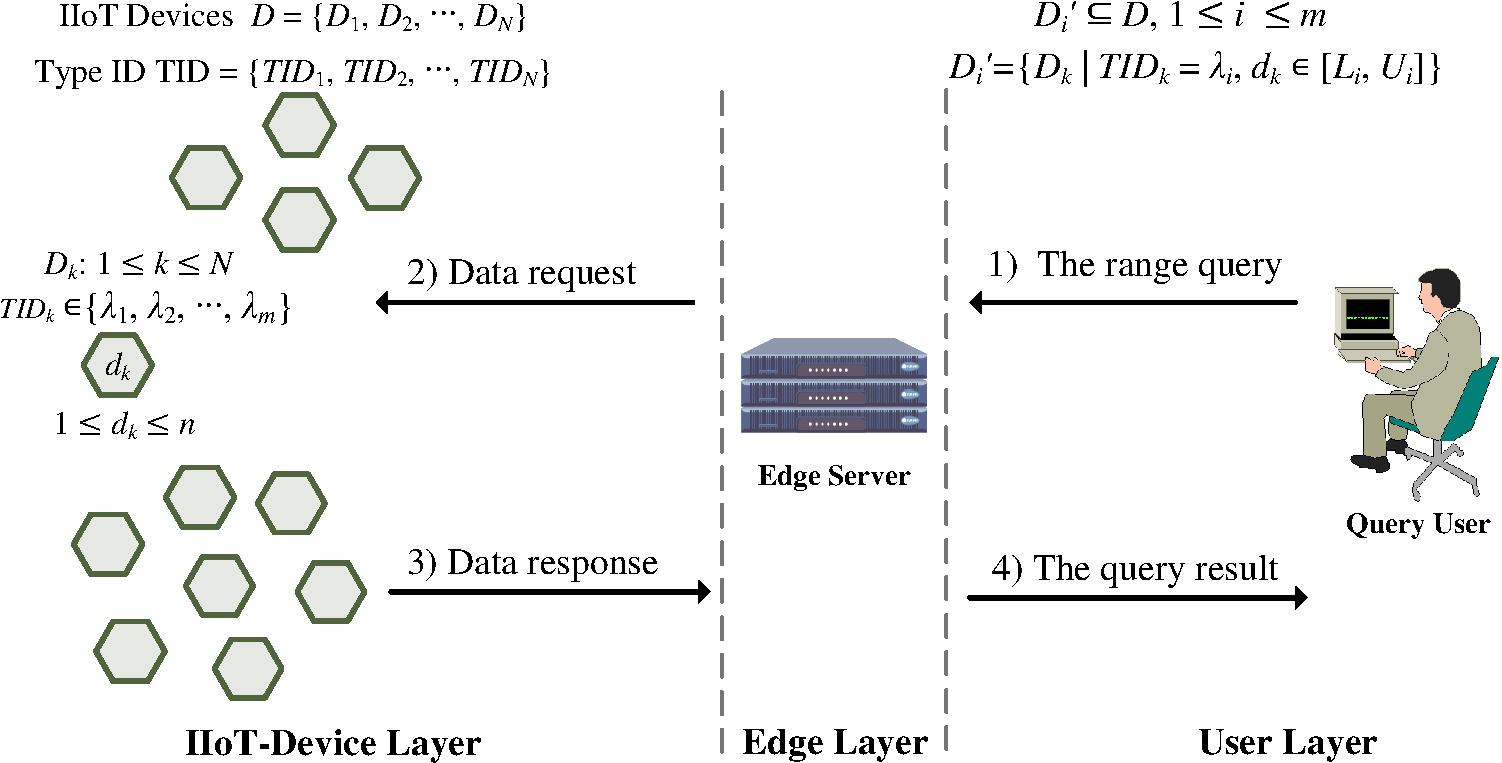
\includegraphics[width=3.3in]{system_model}
  \caption{System model of Edge-PPMRQ}\label{system model}
\end{figure}

\subsection{Security model}
In Edge-PPMRQ, we assume that all entities are honest-but-curious, i.e., each entity performs \textcolor{blue}{the protocol honestly,} but \textcolor{blue}{it} also \textcolor{blue}{wants} to reveal the privacy of other entities. For example, \textcolor{blue}{IIoT} devices and the edge server are curious about the query ranges $[L_i, U_i]$ and the corresponding query results $|D'_i|$, where $1 \le i \le m$; the edge server and the query user are also curious about the sensed data $d_k$ of \textcolor{blue}{IIoT} device $D_k$. This paper focuses on  the \textcolor{blue}{problem} of the privacy-preserving multi-dimensional range query. Similar to the preview work, we assume that there is no collusion among the entities. Meanwhile, we don't consider active attacks of external \textcolor{blue}{adversaries}, which will be discussed in future work.

\subsection{Design goals}
Based on the aforementioned system and security models, a privacy-preserving multi-dimensional range query scheme for edge-supported IIoT should achieve the following goals:
\begin{enumerate}

	\item \emph{Multi-dimensional range query}: Most of traditional range query schemes only support the single-dimensional range query \textcolor{blue}{through} a query request, while the multi-dimensional range query scheme can realize the query for multi-dimensional data by only one query request.

	\item\emph{\textcolor{blue}{Privacy preservation}}: The query ranges $[L_i, U_i]$ and the query \textcolor{blue}{results} $|D'_i|,\ i \in [1, m]$,  cannot be revealed by any other entities except the query user. Besides, the edge server and the query user \textcolor{blue}{can get neither IIoT devices' plaintext of sensed data nor the fact that} if the sensed data of \textcolor{blue}{IIoT} devices is within the query ranges.	
	\item \emph{Continuous, discontinuous and \textcolor{blue}{arbitrary-boundary} range query}:
	Most of the traditional range query schemes only support continuous range query, while in reality, the query ranges may be discontinuous and \textcolor{blue}{have} arbitrary boundary. Consequently, it is very necessary for the multi-dimensional range query schemes to support all the three types of range queries.
	
	\item \emph{\textcolor{blue}{Efficient communication and computation}}: Compared to single-dimensional range query schemes, a multi-dimensional range query scheme should achieve the multi-dimensional range query \textcolor{blue}{more efficiently in terms of communication and computation.} Especially in edge-supported IIoT, the communication \textcolor{blue}{overhead} and \textcolor{blue}{computational costs} of \textcolor{blue}{IIoT} side should be \textcolor{blue}{reduced} as much as possible.
\end{enumerate}

\section{The Proposed Scheme: Edge-PPMRQ}
In this section, \textcolor{blue}{it introduces} a privacy-preserving multi-dimensional range query scheme for edge-supported IIoT (Edge-PPMRQ). Before the detailed description of the scheme, \textcolor{blue}{our designed range division algorithm is first presented,} which is a \textcolor{blue}{crucial} technology in Edge-PPMRQ. Besides, the notations used in Edge-PPMRQ are listed in Table \ref{Notations}.

\begin{table}[h]
	\centering\caption{Notations}
	\label{Notations}
	\begin{tabular}{ll} %% this creates two columns
		\hline
		Notation           & Description\\
		\hline
		$N$                & The number of \textcolor{blue}{IIoT} devices\\
		$n$                & The maximum value of \textcolor{blue}{IIoT} devices' sensed data \\
		$d$                & The data \textcolor{blue}{in the example, $d\in [1, n]$}\\
		$D_k, d_k$         & The $k$-th \textcolor{blue}{IIoT} device and its sensed data, $1 \le k \le N$ \\
		$m$                & The number of query dimensions  \\
		$t$                & The number of query sub-ranges  \\
		$\textcolor{blue}{\lambda_i}$   & \textcolor{blue}{The index of $i$-th dimension, $i\in[1, m]$}\\
		$\lambda$          & The set of $\lambda_i$\\
		$TID_i$            & The dimension identifier of $D_i$'s sensed data\\
		$TID$              & The set of $TID_i$\\
		$[L_i, U_i]$       & The query range for $i$-th dimension data\\
		$[l_j, u_j]$       & The $j$-th query sub-range \\
		$\textcolor{blue}{Q_1, Q_2}$ & \textcolor{blue}{The set of all boundaries in query ranges.} \\
		$D'_i$             & The set of \textcolor{blue}{IIoT} devices, whose sensed data is in $[L_i, U_i]$\\
		$\textcolor{blue}{|D'_i|}$ & \textcolor{blue}{The number of elements in set $D'_i$}\\
		$\textcolor{blue}{D'}$  & \textcolor{blue}{The set of $|D'_i|$, $i\in[1, m]$}\\
		$BF_j$  		   & The $j$-th bloom filter, \textcolor{blue}{$j\in [1, t]$} \\
		$BF$               & The set of bloom filters\\
		$P_f$              & The false positive rate of $BF$\\
		$E_{ij}(r)$        & The cipher of $\lambda_i$'s tab corresponding to $BF_j$, $r\in\{0, 1\}$\\
		$\textcolor{blue}{EM}$             & The set of \textcolor{blue}{ciphertext} $E_{ij}(r)$\\
		$C_{ij}$           &  The $\lambda_i$'s counter corresponding to $BF_j$\\
		$\textcolor{blue}{C}$                & The set of \textcolor{blue}{counter} $C_{ij}$\\
		$\kappa$           & The security parameter to establish \textcolor{blue}{OU cryptosystem}\\
		$pk, sk$           & The public key and \textcolor{blue}{the} private key of \textcolor{blue}{OU cryptosystem}\\
		$s$                & The number of elements mapped into bloom \textcolor{blue}{filters}\\
		$s_j$              & The length of sub-range $[l_j, u_j]$ \\
		$p$ 			   & A large prime number\\
		$g$ 			   & A primitive root of $Z^{*}_p$\\
		$a, g^a$ 		   & The query user's private and public parameters\\
		$b, g^b$ 		   & The \textcolor{blue}{IIoT} devices' private and public parameters\\
		$g^{ab}$           & The key shared among query user and \textcolor{blue}{IIoT} devices\\
		$h$                & A public hash function\\
		$h_k$              & The keyed hash value of $d_k$, i.e., $h(g^{ab} \| d_k)$\\
		\hline
	\end{tabular}
\end{table}


\subsection{\textcolor{blue}{Range} division algorithm}\label{sections division}
In order to achieve the multi-dimensional range query, multi-dimensional query ranges should be processed by the \textcolor{blue}{range} division algorithm as the following steps, \textcolor{blue}{which is also shown in Algorithm \ref{algorithm}}.
\begin{enumerate}
	\item \emph{Query \textcolor{blue}{boundary} extraction:} Suppose that $[L_1, U_1]$, $ [L_2, U_2],... ,$ and $[L_m, U_m]$ represent the query ranges of $m$ dimensions $\lambda_1, \lambda_2, ... ,$ and $\lambda_m$, respectively. For $\forall i$ $\in$ $ [1, m]$, $ 1 \le L_i \le U_i \le n$. Then, all the lower \textcolor{blue}{boundaries} and upper \textcolor{blue}{boundaries} are extracted to a set $Q_1=\{L_1 , U_1, L_2, U_2, ... , L_m, U_m\}$. After that, both the minimum value 1 and maximum value $n$ are inserted into $Q_1$. Finally, $Q_1=\{1, L_1 , U_1, L_2, U_2, ... , L_m, U_m, n\}$.
	\item \emph{Query \textcolor{blue}{boundary} sort}: In order to make the \textcolor{blue}{range} division easier, set $Q_1$ is sorted from smallest to largest and the repeated \textcolor{blue}{boundaries} \textcolor{blue}{in $Q_1$} are deleted. Finally, a sorted set $Q_2=\{l_1, l_2, ... , l_t, l_{t+1}\}$ is generated \textcolor{blue}{from $Q_1$}, where $l_1=1, l_{t+1}=n, l_j < l_{j+1}$ and $j \in [1, t]$.
	\item \emph{Query sub-ranges generation:} According to $Q_2$, $t$ sub-ranges are generated, i.e., $[l_1, l_2]$, $[l_2, l_3]$, $... $, and $[l_t, l_{t+1}]$. For clarity, we denote the sub-ranges as $[l_1, u_1]$, $[l_2, u_2]$, $... $, and $[l_t, u_t]$. Furthermore, the \textcolor{blue}{boundaries} should be adjusted by adding $1$, subtracting $1$ or remaining unchanged to get \textcolor{blue}{the} final sub-ranges $[l_1', u_1']$, $[l_2', u_2']$, $... $, and $[l_t', u_t'
	]$, and the following two conditions should be satisfied for \textcolor{blue}{all query ranges} $[L_i, U_i]$, $1\le i \le m$:
	\begin{enumerate}
		\item $\exists a, b, 1 \le a \le b \le t, [l_a',u_a'] \cup [l_{a+1}', u_{a+1}'] \cup ...  \cup [l_b', u_b'] = [L_i, U_i]$, where $l_a' = L_i$ and $u_b'=U_i$.
		\item $\forall v,w \in [a, b]$, $v \neq w$, $[l_v', u_v']\cap [l_w', u_w'] = \emptyset$.
	\end{enumerate}	
\end{enumerate}

\iffalse
\begin{algorithm}[htb]  
	\caption{ \textcolor{blue}{Range} division algorithm.}  
	\label{algorithm1}  
	\begin{algorithmic}[1]  
		\Require  
		%The set of positive samples for current batch, $P_n$;  
		%The set of unlabelled samples for current batch, $U_n$;  
		%Ensemble of classifiers on former batches, $E_{n-1}$;  
		Query ranges $[L_1, U_1], [L_2, U_2], ..., [L_m, U_m]$ of $m$ dimensions $\lambda_1, \lambda_2, ..., \lambda_m$, respectively. 
		\Ensure  
		%Ensemble of classifiers on the current batch, $E_n$;
		$t$ query sub-ranges $[l_1, u_1], [l_2, u_2], ..., [l_t, u_t]$.  
		\State %Extracting the set of reliable negative and/or positive samples $T_n$ from $U_n$ with help of $P_n$;
		Extracting all the lower and upper \textcolor{blue}{boundaries} of $m$ query ranges to generate a set $Q_1$ $=$$\{$$L_1,$ $U_1,$ $L_2,$ $U_2,$ $ ...,$ $L_m, U_m\}$.  
		%\label{initializing Q1}  
		\State Inserting minimum value $1$ and maximum value $n$ to get the renewed $Q_1$$=$$\{$$1,$ $L_1,$ $U_1,$ $L_2,$ $U_2,$ $...,$ $L_m, U_m, n\}$.  
		%\label{renewing Q1}  
		\State Sorting $Q_1$ from smallest to largest and deleting repeat \textcolor{blue}{boundaries} to generate a sorted set $Q_2$$=$$\{$$l_1,$ $l_2,$ $ ...,$ $l_t,$ $l_{t+1}$$\}$, where $l_1=1, l_t=n$ and $l_j < l_{j+1}, j\in[1, t]$.
		  
		%\label{code:fram:add}  
		\State Generating $t$ ranges $[l_1, l_2], [l_2, l_3], ..., [l_t, l_{t+1}]$ according to $Q_2$ and representing them as $[l_1, u_1], [l_2, u_2], ..., [l_t, u_t]$.    
		\State Adjusting the \textcolor{blue}{boundaries} of $t$ ranges by adding 1, subtracting 1 or remaining unchanged to get final $t$ sub-ranges $[l'_1, u'_1], [l'_2, u'_2], ..., [l'_t, u'_t]$, which meet two conditions: 
		\begin{enumerate}
			\item $\exists a, b, 1 \le a \le b \le t, [l_a',u_a'] \cup [l_{a+1}', u_{a+1}'] \cup ...  \cup [l_b', u_b'] = [L_i, U_i]$, where $l_a' = L_i$ and $u_b'=U_i$.
			\item $\forall v,w \in [a, b]$, $v \neq w$, $[l_v', u_v']\cap [l_w', u_w'] = \emptyset$.
		\end{enumerate}	
		  \\  
		\Return $t$ query sub-ranges $[l'_1, u'_1], [l'_2, u'_2], ..., [l'_t, u'_t]$.  
	\end{algorithmic}  
\end{algorithm}  
\fi


\begin{algorithm}[h]  
	\caption{\textcolor{blue}{Range division algorithm}.}
	\label{algorithm}  
	\begin{algorithmic}[1]
		\Require  
		%The set of positive samples for current batch, $P_n$;  
		%The set of unlabelled samples for current batch, $U_n$;  
		%Ensemble of classifiers on former batches, $E_{n-1}$;  
		\textcolor{blue}{Query ranges $[L_1, U_1], [L_2, U_2], ..., [L_m, U_m]$ of $m$ dimensions $\lambda_1, \lambda_2, ..., \lambda_m$ and maximum value of range $n$.} 
		\Ensure \textcolor{blue}{the set of $t$ query sub-ranges $[l_1, u_1]$, $[l_2, u_2]$, ..., $[l_t, u_t]$, i.e., $Q_2$.}  
		\State \textcolor{blue}{Initialize $Q_l, Q_u, Q_1, Q_2$ to empty arrays;}
		\State \textcolor{blue}{Insert $1$ into $Q_l$;}
		\State \textcolor{blue}{Insert $n$ into $Q_u$;}
		\State \textcolor{blue}{Insert $1, n$ into $Q_1$;}
		\For{\textcolor{blue}{each $i\in [1,m]$}}
		\State \textcolor{blue}{insert $L_i$ into $Q_l$;}
		\State \textcolor{blue}{insert $U_i$ into $Q_u$;}
		\State \textcolor{blue}{insert $L_i$, $U_i$ into $Q_1$;}   
		\EndFor 
		\State \textcolor{blue}{$//$ $Q_l=[1, L_1, L_2, ..., L_m]$;}
		\State \textcolor{blue}{$//$ $Q_u=[n, U_1, U_2, ..., U_m]$;}
		\State \textcolor{blue}{$//$ $Q_1=[1, n, L_1, U_1, L_2, U_2, ..., L_m, U_m]$;}
		\State \textcolor{blue}{De-duplication $(Q_1)$;}
		\State \textcolor{blue}{Sort $(Q_1)$ from smallest to biggest;}
		\State \textcolor{blue}{$//$ $Q_1=[l_1, l_2, ..., l_t, l_{t+1}]$, where $l_1=1$ and $l_{t+1}=n$;}
		%\State Let $Q_2=Q_1;$
		\For{\textcolor{blue}{each $j \in [1, t]$}}
		\State \textcolor{blue}{extract $l_j, l_{j+1}$ from $Q_1$;}
		\State \textcolor{blue}{generate range $[l_j, l_{j+1}]$;}
		\State \textcolor{blue}{represent range $[l_j, l_{j+1}]$ as $[l_j, u_j]$;}
		\State \textcolor{blue}{insert $[l_j, u_j]$ into $Q_2$;}
		\EndFor
		\For {\textcolor{blue}{each $j \in [1, t]$}}
		\State \textcolor{blue}{extract $[l_j, u_j], [l_{j+1}, u_{j+1}]$ from $Q_2$;}
		\While {\textcolor{blue}{$[l_j, u_{j}] \cap [l_{j+1}, u_{j+1}] \neq \emptyset$}}
		%\If {$u_j \in Q_l \cap Q_u$}
		%\State insert $[u_j, u_j]$ into $Q_2$;
		%\EndIf
		\If {\textcolor{blue}{$u_j \in Q_l$}}
		\State \textcolor{blue}{$u_j=u_j-1$}
		\EndIf
		\If {\textcolor{blue}{$u_j \in Q_u$}}
		\State \textcolor{blue}{$l_{j+1}=l_{j+1}+1$}
		\EndIf
		\EndWhile
		\State \textcolor{blue}{insert $[l_j, u_j], [l_{j+1}, u_{j+1}]$ into $Q_2$;}
		\EndFor\\
		\Return \textcolor{blue}{$Q_2$.}    
	\end{algorithmic}  
\end{algorithm} 


To better understand \textcolor{blue}{the} proposed \textcolor{blue}{range} division algorithm, we give a toy example here, which is also shown in Fig. \ref{sections division algorithm}. For $n = 100, m = 2$ and two dimensions $\lambda_1$ and $\lambda_2$ with the corresponding query ranges $[20, 60]$ and $[40, 80]$, respectively, the query sub-ranges can be generated by the above \textcolor{blue}{range} division algorithm:
\begin{enumerate}
	\item According to \textcolor{blue}{ranges} $[20, 60]$ and $[40, 80]$, \textcolor{blue}{it gets set $Q_1=\{1, 20, 60, 40, 80, 100\}$.}
	\item Based on $Q_1$, \textcolor{blue}{it gets the sorted set $Q_2=\{1, 20, 40, 60, 80, 100\}$.}
	\item Then \textcolor{blue}{it gets} $5$ sub-ranges $[1, 20], [20, 40], [40, 60],$ $[60, 80]$ and $[80, 100]$. Moreover, the boundaries of the sub-ranges are adjusted to generate the final sub-ranges $[1, 19], [20, 39], [40, 60], [61, 80]$ and $[81, 100]$.	
From the sub-ranges, we can see that:
	\begin{enumerate}
		\item $[20,39] \cup [40, 60] = [20, 60]$ and $[40, 60] \cup [61, 80]=[40, 80]$.
		\item $[20,39] \cap [40, 60] = \emptyset$ and $[40, 60] \cap [61, 80]= \emptyset$.
	\end{enumerate}
\end{enumerate}

\textcolor{blue}{It is worth noting that different types of data may locate in ranges with great distance, which exist very small or even no overlap. However, different kinds of data, such as the temperature and pressure, have different accuracy requirements. When the sensed data is transformed into integers based on the aforementioned method, the \textcolor{blue}{corresponding} ranges may have some overlap. For example, the query ranges of temperature values and pressure values are $[120.5, 200.5]$ and $[1000, 1800]$, respectively. Then, the ranges will be transformed into $[1205, 2005]$ and $[1000, 1800]$ and they have a big overlap $[1205, 1800]$, which is helpful for our scheme. Therefore, in this situation, our scheme can also achieve efficient communication performance.} 




\begin{figure}
	\centering
	% Requires \usepackage{graphicx}
	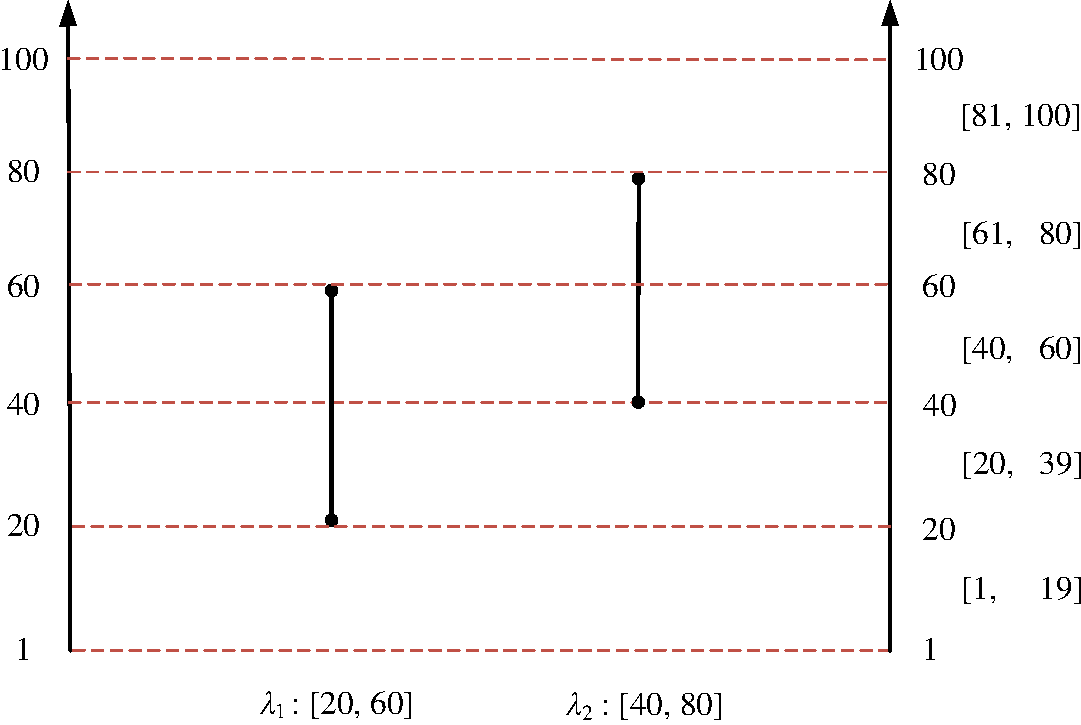
\includegraphics[width=3.4in]{ranges_division_model}\\
	\caption{An example of \textcolor{blue}{range} division algorithm}\label{sections division algorithm}
\end{figure}


\subsection{Description of Edge-PPMRQ}
 \textcolor{blue}{Our privacy-preserving multi-dimensional range query scheme for edge-supported IIoT (Edge-PPMRQ) is described in detail as below.}

\subsubsection{System initialization}
To initialize the system, the service provider selects a hash function $h$, a large prime number $p$, a primitive root $g\in Z^*_p$ and a random number $b\in Z^*_p$. Then, $g^b$ mod $p$ can be computed accordingly. Finally, the service provider publishes the parameters $h, p, g$ and $g^b$. After that, the service provider deploys an edge server and various \textcolor{blue}{types of IIoT} devices to the target industrial environment.

\subsubsection{User query request generation}
The query user launches a query for data of $m$ dimensions $\lambda =\{\lambda_1, \lambda_2, ... , \lambda_m\}$, i.e., ``How many \textcolor{blue}{IIoT} devices of dimension $\lambda_i$, whose sensed data $d_k$ is within range $[L_i, U_i]$, where $1 \le i \le m$ and $1 \le k \le N$?"  In other words, the query user would like to figure out: For $\forall i \in [1, m]$ and $ k \in [1, N]$, $|D_i'|=Count(D'_i)$, where $D'_i=\{D_k | TID_k=\lambda_i$, $d_k \in [L_i, U_i]\}$. To generate the query request in a privacy-preserving way, the query user performs the following steps.

\textbf{Step 1}: Given a security parameter $\kappa$, \textcolor{blue}{the public and private key pair $(pk, sk)$ of OU cryptosystem is generated by the key generation algorithm.} Besides, a random number $a\in Z_p^*$ is chosen to compute $g^a$ mod $p$ and $g^{ab}=(g^b)^a$ mod $p$.
	
\textbf{Step 2}: For $m$ query ranges $[L_1, U_1], [L_2, U_2], ... ,$ and $[L_m, U_m]$ corresponding to dimensions $\lambda_1, \lambda_2, ...,$ and $\lambda_m$, respectively, the \textcolor{blue}{range} division algorithm is called to output $t$ query sub-ranges $[l_1, u_1], [l_2, u_2], ... ,$ and $[l_t, u_t]$.

\textbf{Step 3}: A group of $t$ bloom filters with $n$-bit vectors and $k$ hash functions are chosen. Here, for each bloom filter, $s$, i.e. the number of mapped elements, should satisfy $s \le \lceil \frac{n}{{\rm log}n} \rceil $ and $k$ should meet $k=\frac{n}{s}{\rm ln}2$ to ensure the false positive rate $P_f=(1-(1-\frac{1}{n})^{ks})^k \approx (1-e^{-\frac{ks}{n}})^k  =n^{-{\rm ln}2}$.

\textbf{Step 4}: For each sub-range $[l_j, u_j]$, $1<$$j$$<t$, all integers between $l_j$ and $u_j$ are mapped into $BF_j$. Note that, we don't map the integer value $d\in [l_j, u_j]$ itself but its keyed hash value $h(g^{ab}\|d)$ into $BF_j$. For sub-range $[l_i, u_i]$ with length $s_i$, where $1 \le i \le t$, if $s_i  >\lceil \frac{n}{{\rm log} n} \rceil$, we divide it into some shorter sub-ranges to ensure the false positive rate. For simplicity, we assume that the length $s_i$ is smaller than $\lceil \frac{n}{{\rm log} n} \rceil$.

\textbf{Step 5}: For dimension $\lambda_i$, the query user constructs a query set $\{BF_j, E_{ij}(r), C_{ij}\}$, where $i\in [1, m]$, $j \in [1, t]$ and $r \in \{0, 1\}$. $BF_j$ is the bloom filter which the $j$-th sub-range $[l_j, u_j]$ is mapped into. $E_{ij}(r)$ is the OU ciphertext of $r$, where $r$ is a label to indicate the relationship between the $i$-th dimension $\lambda_i$ and the $j$-th bloom filter $BF_j$. Concretely, if the $j$-th sub-range $[l_j, u_j]$ (mapped into $BF_j$) is a sub-set of the dimension $\lambda_i$'s query range $[L_i, U_i]$, the $r$ is labeled as $1$ $(E_{ij}(r)=E(1))$; otherwise, $r$ is set as $0$ $(E_{ij}(r)=E(0))$.  $C_{ij}$ is a counter with initial value $0$, which is used to record how many \textcolor{blue}{IIoT} devices of dimension $\lambda_i$, whose sensed data is in the $j$-th sub-range $[l_j, u_j]$. Finally, we get:
	$$EM = {\left [\begin{array}{cccc}
					E_{11}(r) & E_{12}(r) & \cdots & E_{1t}(r)\\
					E_{21}(r) & E_{22}(r) & \cdots & E_{2t}(r)\\
					\vdots    & \vdots    & \ddots & \vdots\\
					E_{m1}(r) & E_{m2}(r) & \cdots & E_{mt}(r)
					\end{array} \right] },$$
	%\vspace{-0.14cm}			
	$$C= \left [
		\begin{array}{cccc}
			C_{11} & C_{12} & \cdots & C_{1t}\\
			C_{21} & C_{22} & \cdots & C_{2t}\\
			\vdots & \vdots  & \ddots & \vdots\\
			C_{m1} & C_{m2} & \cdots & C_{mt}
		\end{array}	
		\right].$$
		
\textbf{Step 6}: As shown in Fig. \ref{query request}, the query user constructs a query request $\{\lambda, BF, EM, C, g^a$ mod $p\}$, where $\lambda=\{\lambda_1, \lambda_2, ..., \lambda_m\}$ and $BF=\{BF_1, BF_2, ..., BF_t\}$. Then the query request is sent to the edge server. Accordingly, the edge server broadcasts $\{\lambda,  g^a$ mod $p\}$ to all \textcolor{blue}{IIoT} devices.

	\begin{figure}
		\centering
		% Requires \usepackage{graphicx}
		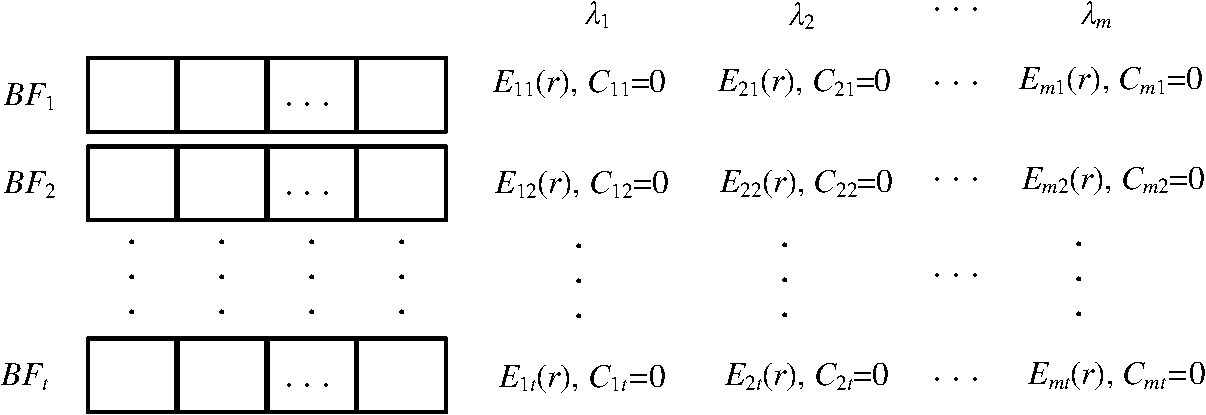
\includegraphics[width=3.4in]{query_request_model}\\
		\caption{Query request generation}\label{query request}
	\end{figure}
	

 Based on the example given in \textcolor{blue}{range} division algorithm, \textcolor{blue}{the concrete process of the user query request generation algorithm is shown as below:} \label{example}
 	\begin{enumerate}
 		\item For the $5$ sub-ranges $[1, 19], [20, 39], [40, 60] $, $[61 , 80]$ and $[81, 100]$ generated \textcolor{blue}{in the example of \ref{sections division}}, all the values in the sub-ranges \textcolor{blue}{are mapped into} $5$ bloom filters $BF_1,BF_2,BF_3,BF_4$ and $BF_5$, respectively. For instance, all the values $1, 2, ..., $ and $ 19$ in the sub-range $[1, 19]$ are mapped into $BF_1$.
 		\item For the query range $[20, 60]$ of dimension $\lambda_1$, only $[20, 39]$ and $[40, 60]$ are its sub-sets. Therefore, only $E_{12}(r)$ and $E_{13}(r)$ are $1$. Then, the query user constructs a query set $\{BF_j, E_{1j}(r), C_{1j}\}$, $j\in [1, 5]$ and $r \in \{0,1\}$, i.e., $\{\{BF_1, BF_2,BF_3,$ $ BF_4, BF_5\}, \{E_{11}(0),E_{12}(1), E_{13}(1), E_{14}(0), E_{15}(0)\},$ $ \{C_{11}, C_{12}, C_{13}, C_{14}, C_{15}\}\}$. Similarly, for the query range $[40, 80]$ of dimension $\lambda_2$, the query user can also generate \textcolor{blue}{a} query set correspondingly. Finally, the query request, i.e., two query sets, is generated as shown in Fig. \ref{query_request_example}.
 	\end{enumerate}
 	
 \begin{figure}
 	\centering
 	% Requires \usepackage{graphicx}
 	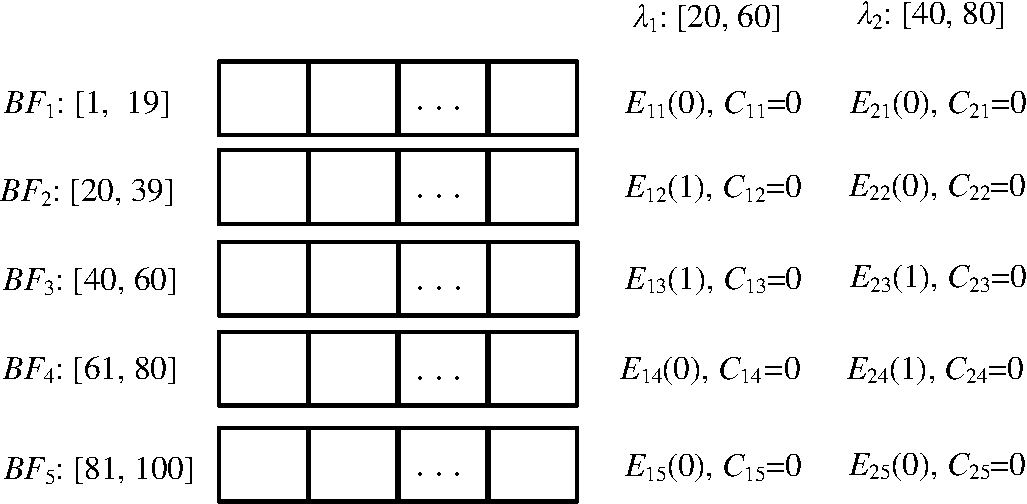
\includegraphics[width=3.4in]{query_request_example}\\
 	\caption{An example of query request}\label{query_request_example}
 \end{figure}

\subsubsection{\textcolor{blue}{IIoT} devices' data response}
 When receiving the data request $\{\lambda,  g^a$ mod $p\}$ forwarded by the edge server, each \textcolor{blue}{IIoT} device $D_k$ $\in D$ checks if its type ID $TID_k$ is in the queried dimensions $\lambda=\{\lambda_1, \lambda_2, ..., \lambda_m\}$. If $TID_k$ doesn't belong to $\lambda$, $D_k$ discards the data request. Otherwise, $D_k$ computes the shared key $g^{ab}$ mod $p$ by using $b$ and $g^a$ mod $p$. Then, $D_k$ computes the
  keyed hash value $h_k=h(g^{ab} \| d_k)$. Finally, $\{TID_k, h_k\}$ is responded to the edge server via a secure channel.

\subsubsection{Edge server's data aggregation}
Upon receiving all the responses $\{TID_k, h_k\}, k\in [1, N]$ from \textcolor{blue}{IIoT} devices, the edge server performs the following steps to aggregate the data.

\textbf{Step 1}: Edge server takes $TID_k$ from $\{TID_k, h_k\}$ and find the corresponding query dimension $\lambda_i$ from $\lambda$, where $1\le i \le m$.

\textbf{Step 2}: Edge server takes $h_k$ from $\{TID_k, h_k\}$ and checks if $h_k$ is in $BF_j$, where $BF_j \in BF$ and $j \in [1, t]$. If so, the counter $C_{ij}$ increases by $1$. Otherwise, $C_{ij}$ keeps unchanged.

\textbf{Step 3}: After the above processes, the edge server aggregates the data as $C_i = \prod_{j=1}^{t}(E_{ij}(r)^{C_{ij}})$, where $1\le i \le m$, and responses the results $C=\{C_1, C_2, ... ,C_m\}$ to the query user.


  Following the last example \textcolor{blue}{in section \ref{example}}, suppose that the data responses from \textcolor{blue}{IIoT} devices are 
 \label{example2} $\{\lambda_1,h(g^{ab}\|5)\},$ $ \{\lambda_1, h(g^{ab}\|20)\},$ $ \{\lambda_1, h(g^{ab}\|30)\},$ $ \{\lambda_2, h(g^{ab}\|35)\},$ $ \{\lambda_2, h(g^{ab}\|45)\}, $ $ \{\lambda_1, h(g^{ab}\|50)\}, $ $ \{\lambda_1, h(g^{ab}\|55)\},$ $ \{\lambda_2, h(g^{ab}\|55)\}, $ $ \{\lambda_2, h(g^{ab}\|65)\}, $ $ \{\lambda_2, h(g^{ab}\|90)\}$. The edge server performs the steps as below to aggregate the sensed data.

  \textbf{Step 1}: When receiving the data responses, the edge server \textcolor{blue}{classifies} the dimension $\lambda_1$'s sensed data $h(g^{ab}\|5), h(g^{ab}\|20),$ $ h(g^{ab}\|30)$, $h(g^{ab}\|50)$ and $h(g^{ab}\|55)$, and $\lambda_2$'s sensed data $h(g^{ab}\|35), h(g^{ab}\|45),$ $ h(g^{ab}\|55), h(g^{ab}\|65)$ and $h(g^{ab}\|90)$.

  \textbf{Step 2}: It checks the bloom filter which the sensed data belongs to and increases the corresponding counter, e.g., $h(g^{ab}\|5)$ of $\lambda_1$ is \textcolor{blue}{checked in} $BF_1$, so the corresponding counter $C_{11}$ increases by $1$. Finally, the counters $C_{11}=1, C_{12}=2, C_{13}=2,C_{14}=0, C_{15}=0, C_{21}=0, C_{22}=1, C_{23}=2$, $C_{24}=1$ and $C_{25}=1$.

  \textbf{Step 3}: According to $E_{11}(0),E_{12}(1), E_{13}(1),E_{14}(0), E_{15}(0),$ $ E_{21}(0),E_{22}(1), E_{23}(1), E_{24}(0)$ and $E_{25}(0)$ and counters, the data is aggregated as:
  \begin{align*}
  		C_1 &= \prod_{j=1}^{5}(E_{1j}(r)^{C_{1j}})\\
  		    &= E_{11}(0)^{1} \cdot E_{12}(1)^{2} \cdot E_{13}(1)^{2} \cdot E_{14}(0)^{0} \cdot E_{15}(0)^{0} \\
  		    &= E_{11}(0) \cdot E_{12}(2) \cdot E_{13}(2) \cdot 1 \cdot 1\\
  		    &= E(4)\\
  		C_2 &= \prod_{j=1}^{5}(E_{2j}(r)^{C_{2j}})\\
  		    &= E_{21}(0)^{0} \cdot E_{22}(0)^{1} \cdot E_{23}(1)^{2} \cdot E_{24}(1)^{1} \cdot E_{25}(0)^{1} \\
  		    &= 1 \cdot E_{22}(0) \cdot E_{23}(2) \cdot E_{24}(1) \cdot E_{25}(0) \\
  		    &= E(3)\\	
  \end{align*}
  Finally, $C=\{C_1, C_2\}$ is replied to the query user.\\

	


\subsubsection{\textcolor{blue}{Response} recovery}
When receiving $C=\{C_1, C_2,$ $ ..., C_m\}$ from the edge server, the query user recovers the corresponding query results $D'=\{|D'_1|, |D'_2|, ... ,|D'_m|\}$ by decrypting $C$ as
\begin{align*}
|D'_i|= Count(D'_i) = Dec(C_i), 1\le i \le m
\end{align*}

The correctness of the result is shown as
\begin{align*}
	Dec(C_i) &= Dec(\prod_{j=1}^{t}(E_{ij}(r)^{C_{ij}})) \\
&= Dec(\prod_{BF_j\in [L_i, U_i]}(E_{ij}(1)^{C_{ij}}) \cdot \prod_{BF_j \notin [L_i, U_i]}(E_{ij}(0)^{C_{ij}})) \\
&= Dec(E(\sum_{BF_j \in [L_i, U_i]}(1\cdot C_{ij}) + \sum_{BF_j \notin [L_i, U_i]}(0\cdot C_{ij}))) \\
&= Dec(E(\sum_{BF_j \in [L_i, U_i]}C_{ij})) \\
&= \sum_{BF_j \in [L_i, U_i]}C_{ij}\ \ \ \ \ \ \ \ \ \ \ \ \ \ \ \ \ \ \ \ \ \ \ \ \ \ \ \ \ \ \ \ \ \ \ \ \\\
&= |D'_i|.
\end{align*}

\textcolor{blue}{Following the} example \textcolor{blue}{in section \ref{example2}}, when receiving $C=\{C_1, C_2\}$, the query user can recover the query result as:
 \begin{align*}
 |D'_1| &= Count(D'_1) = Dec(C_1)=4. \\
 |D'_2| &= Count(D'_2) = Dec(C_2)=3.
 \end{align*}

 Therefore, the query user knows that there are $4$ \textcolor{blue}{sensors of dimension $\lambda_1$, whose sensed data is in the query range $[20, 60]$ and $3$ sensors of dimension $\lambda_2$, whose sensed data is in the range $[40, 80]$.}

\section{Security Analysis}
In this section, we analyze the security features of Edge-PPMRQ and prove that it achieves the aforementioned security requirements. We especially focus on privacy-preserving properties as below.

\begin{enumerate}
	\item \emph{Query ranges $[L_i, U_i], i\in [1, m]$ are privacy-preserving in Edge-PPMRQ}:
	In order to achieve multi-dimensional range query, the $m$-dimensional query ranges are divided into $t$ sub-ranges by the proposed \textcolor{blue}{range} division algorithm. Then, the sub-ranges are mapped into $t$ bloom filters to generate the query request. Subsequently, the query \textcolor{blue}{user transfers the query request to the edge server} via a public channel. Through the channel, an \textcolor{blue}{IIoT} device $D_k$ can eavesdrop the query request. At the same time, $D_k \in D$ owns shared key $g^{ab}$ mod $p$. Therefore, for $\forall d \in [1, n]$, $D_k$ can compute all keyed hash values $h(g^{ab} \| d)$ and check the bloom filter which $h(g^{ab} \| d)$ belongs to. In such way, $D_k$ can recover the sub-range $[l_j, u_j]$ which is mapped into $BF_j$, $j\in[1, t]$. However, $D_k$ cannot distinguish the ciphertexts of $0$ and $1$ because \textcolor{blue}{OU cryptosystem} is semantically secure \cite{ou1998}, i.e., it cannot know the real value of $r$ in $E_{ij}(r)$. As a result, $D_k$ cannot confirm if the query sub-range $[l_j, u_j]$ is a sub-set of the query range $[L_i, U_i]$. Due to the same reason, even though $D_k$ knows sub-range $[l_j, u_j]$ is mapped into $BF_j$, $D_k$ still cannot get any information about the query range $[L_i, U_i]$ of dimension $\lambda_i$. Besides, \textcolor{blue}{the edge server can neither get shared key $g^{ab}$ mod $p$ nor distinguish the ciphertexts of $0$ and $1$.} Therefore, it cannot get any information about $[l_j, u_j]$ and $[L_i, U_i]$. Based on above analysis, the query ranges $[L_i, U_i]$ of dimension $\lambda_i$, $i \in [1, m]$ are privacy-preserving for \textcolor{blue}{IIoT} devices and the edge server in Edge-PPMRQ.
	
	\item \emph{The query result $D'=\{|D'_1|, |D'_2|, ... , |D'_m|\}$ is also privacy-preserving in Edge-PPMRQ}:
	For the edge server, it receives the query request $\{\lambda, BF, EM, C, g^a$ mod $p\}$ from the query user and the data response $\{TID_k, h_k\}$, $k \in [1, N]$, from \textcolor{blue}{IIoT} devices. Even though it can know the bloom filter which the keyed hash value $h_k=h(g^{ab} \| d_k)$ belongs to,
	it cannot confirm if a sub-range $[l_j, u_j]$, which is mapped into the bloom filter $BF_j$, is the sub-set of the query range $[L_i, U_i]$. \textcolor{blue}{The reason is that} it cannot distinguish the ciphertexts of $0$ and $1$, according to the semantic security of \textcolor{blue}{OU cryptosystem} \cite{ou1998}.
    Therefore, the edge server cannot confirm if the sensed data $d_k$ of \textcolor{blue}{IIoT} device $D_k$ is in the query range $[L_i, U_i]$ of dimension $\lambda_i$, $i\in [1, m]$, i.e., it has no idea about that how many \textcolor{blue}{IIoT} devices whose sensed data is in range $[L_i, U_i]$. In other words, the query result $D'$ is privacy-preserving for the edge server. Besides, each \textcolor{blue}{IIoT} device $D_k \in D$ owns $g^{ab}$ mod $p$ and can compute all keyed hash values of data in $[1, n]$. However, every \textcolor{blue}{IIoT} device transfers its data response via a secure channel. As a result, $D_k$'s sensed data $d_k$ cannot be recovered by other \textcolor{blue}{IIoT} devices. At the same time, $E_{ij}(r)$ is also indistinguishable for \textcolor{blue}{IIoT} devices. Thus, \textcolor{blue}{IIoT} devices have no way to know the query result $D'$. Based on the above analysis, we prove that the query result $D'$ is privacy-preserving for the edge server and \textcolor{blue}{IIoT} devices.
	
	\item \emph{Plaintext data $d_k$ of \textcolor{blue}{IIoT} device $D_k$ is also privacy-preserving in Edge-PPMRQ}:
	For the edge server, it can get $g^a$ mod $p$ from the query request. However, $b$ is the private parameter of \textcolor{blue}{IIoT} devices. Therefore, the edge server cannot compute $g^{ab}$ mod $p$. In other words, it cannot recover $d_k$ from $h_k=h(g^{ab}\| d_k)$. Similar to some previous work, in our model, the \textcolor{blue}{IIoT} devices send their data response via a secure channel. As a result, $D_k$'s sensed data $d_k$ cannot be recovered by other \textcolor{blue}{IIoT} devices. Likewise, the query user also cannot recover the sensed data of \textcolor{blue}{IIoT} devices. Based on the above analysis, the plaintext data $d_k$ of \textcolor{blue}{IIoT} device $D_k$ is also privacy-preserving.
\end{enumerate}


\section{Performance Evaluation}

In this section, we evaluate the performance of Edge-PPMRQ and three related work, i.e., BFPRQ \cite{mahdikhani2020IoT}, CEPRQ \cite{hasan2020IoT} and URPRQ \cite{mahdikhani2020using} from the aspects of communication overhead and computational cost. Here, it should be noted that Edge-PPMRQ and BFPRQ \cite{mahdikhani2020IoT} are based on \textcolor{blue}{OU cryptosystem} \cite{ou1998} and \textcolor{blue}{Paillier cryptosystem} \cite{paillier1999}, respectively, while CEPRQ \cite{hasan2020IoT} and URPRQ \cite{mahdikhani2020using} are based on their own constructed homomorphic encryption SHE. All the schemes are simulated with Python 3.8, Gmpy 2 and Math library. The experiments are carried out on an Intel(R) Core (TM) i5-7400 CPU @3.00GHz with Windows 10 system and 24GB RAM. To ensure the fairness, we keep the false positive rate of bloom filters in BFPRQ \cite{mahdikhani2020IoT} and Edge-PPMRQ as $n^{-\rm{ln}2}$. Besides, we simulate $m$-dimensional range query of BFPRQ \cite{mahdikhani2020IoT}, CEPRQ \cite{hasan2020IoT} and URPRQ \cite{mahdikhani2020using} by performing $m$ single-dimensional query requests since they don't support multi-dimensional range query. Furthermore, we evaluate \textcolor{blue}{and compare} the communication overhead and computational cost of \textcolor{blue}{these} four schemes in two conditions: (1) $n$ is varying from $2^{10}$ to $2^{20}$, while $m$ is fixed at 16; (2) $m$ is varying from $5$ to $55$, while $n$ is fixed at $2^{20}$. In addition, the detailed parameters setting and notations used in the comparison are shown in Table \ref{parameters table}.

\begin{table}
\centering\caption{The parameters setting and notations}
\label{parameters table}
\begin{tabular}{lll}
\hline
Parameter & Value \\
\hline
$\kappa$ & $\kappa=512, |p|=|q|=\kappa$\\
$h$ &The public hash function SHA-256\\
$k$ &The number of hash functions $k$= $\rm{log}$$n$$ \times\rm{ln}2$ \\
$N$ &The number of single dimension's \textcolor{blue}{IIoT} devices. $N$=$1000$ \\
$|\lambda_i|$ & The length of dimension index with the length of $6$ bits\\
$m$ & The number of dimensions in the query request\\
$b$ & $\rm{log}$$n$\\
$|E_{paillier}|$ & The length of paillier ciphertext\\
$|E_{SHE}|$ & The length of SHE ciphertext\\
$|E_{OU}|$ & The length of OU ciphertext\\
$|H|$ & The length of SHA-256's output\\
\hline
\end{tabular}
\end{table}


\iffalse
\begin{figure*}[htbp]	
	\centering
	\begin{subfigure}[t]{0.3\textwidth}
		\centering
		\includegraphics[width=1\textwidth]{commu1_m}\\
		\caption{Communication overhead of user side}\label{user side communication}	
	\end{subfigure}
	\quad
	\begin{subfigure}[t]{0.3\textwidth}
		\centering
		\includegraphics[width=1\textwidth]{commu2_m}\\
		\caption{Communication overhead of \textcolor{blue}{IIoT} side}\label{IoT side communication}
	\end{subfigure}
	\caption{Communication overhead comparison with varying $m$}\label{communication_m}
\end{figure*}
\fi


  \begin{table*}
	\caption{Communication overhead between the edge server and the query user with varying $n$}\label{commu_1_n}
	\begin{center}
		\begin{tabular}{ l  l  l  l }
			\hline
			Schemes  & Query request (bits)& Query result (bits)& Total overhead (bits) \\ \hline
			BFPRQ    & $m \cdot [b \cdot (n+|E_{paillier}|)+  |\lambda_i|)]$  & $m \cdot (|E_{paillier}| + |\lambda_i|)$ & $ 16 \cdot b \cdot n + 32768 \cdot b + 32864$ \\
			CEPRQ       & $m \cdot [(2+\frac{2\cdot b^3+3\cdot b^2-11\cdot b}{6}) \cdot |E_{SHE}| + |\lambda_i|]$ & $m \cdot (|E_{SHE}| + |\lambda_i|) $ & $ \frac{2560}{3}  \cdot b^4 + \frac{6400}{3} \cdot b^3 + \frac{10240}{3} \cdot b^2 + \frac{124160}{3} \cdot b + 46176 $  \\
			URPRQ       & $m \cdot [(b-1) \cdot (b+2) \cdot |E_{SHE}| + |\lambda_i|]$ & $m \cdot (|E_{SHE}|+ |\lambda_i|)$ & $2560 \cdot b^{3} + 2560 \cdot b^{2} + 96$ \\
			Edge-PPMRQ  & $b \cdot (n +m  \cdot |E_{OU}|) + m \cdot |\lambda_i| $     &  $m \cdot (|E_{OU}|+ |\lambda_i|)$  & $b \cdot n + 24576 \times b + 24672$ \\ \hline
		\end{tabular}
	\end{center}
\end{table*}


 \begin{table*}
	\caption{Communication overhead between the edge server and \textcolor{blue}{IIoT} devices with varying $n$}\label{commu_2_n}
	\begin{center}
		\begin{tabular}{ l  l  l  l }
			\hline
			Schemes  & Data request (bits)& Data response (bits)& Total overhead (bits) \\ \hline
			BFPRQ    & $m \cdot |\lambda_i|$  & $m \cdot N \cdot (|H| + |\lambda_i|)$ & $4192096$ \\
			CEPRQ       & $m \cdot [(2+\frac{2\cdot b^3+3\cdot b^2-11\cdot b}{6}) \cdot |E_{SHE}| + |\lambda_i|]$ & $m \cdot N \cdot  (|E_{SHE}| + |\lambda_i|)$ & $ \frac{2560}{3}  \cdot b^4 + \frac{6400}{3} \cdot b^3 + \frac{10240}{3} \cdot b^2 + \frac{124160}{3} \cdot b + 46176 $  \\
			URPRQ       & $m \cdot [(b-1) \cdot (b+2) \cdot |E_{SHE}| + |\lambda_i|]$ & $m \cdot N \cdot  (|E_{SHE}| + |\lambda_i|)$ & $2560 \cdot b^{3} + 2560 \cdot b^{2} + 96$ \\
			Edge-PPMRQ  & $m \cdot |\lambda_i|$   &  $m \cdot N \cdot (|H| + |\lambda_i|)$  & $4192096$ \\ \hline
		\end{tabular}
	\end{center}
\end{table*}



\begin{figure*}%[htbp]	
	\centering
	\begin{subfigure}[t]{0.23\textwidth}
		\centering
		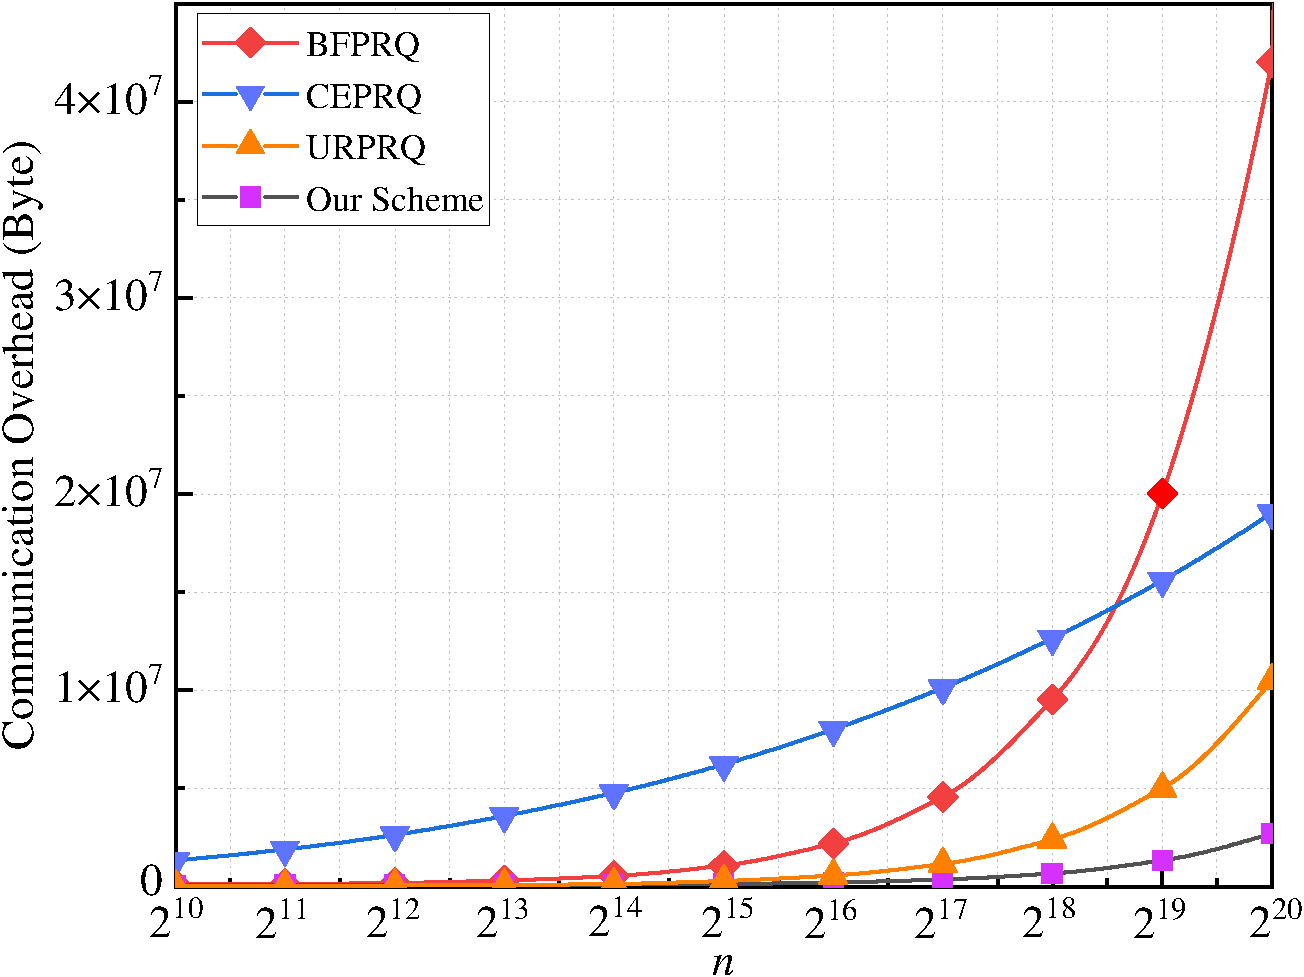
\includegraphics[width=1\textwidth]{commu_1n}\\
		\caption{Between \textcolor{blue}{the} edge server and \textcolor{blue}{the} query user with varying $n$}\label{commu_1n}	
	\end{subfigure}
	\quad
	\begin{subfigure}[t]{0.23\textwidth}
		\centering
		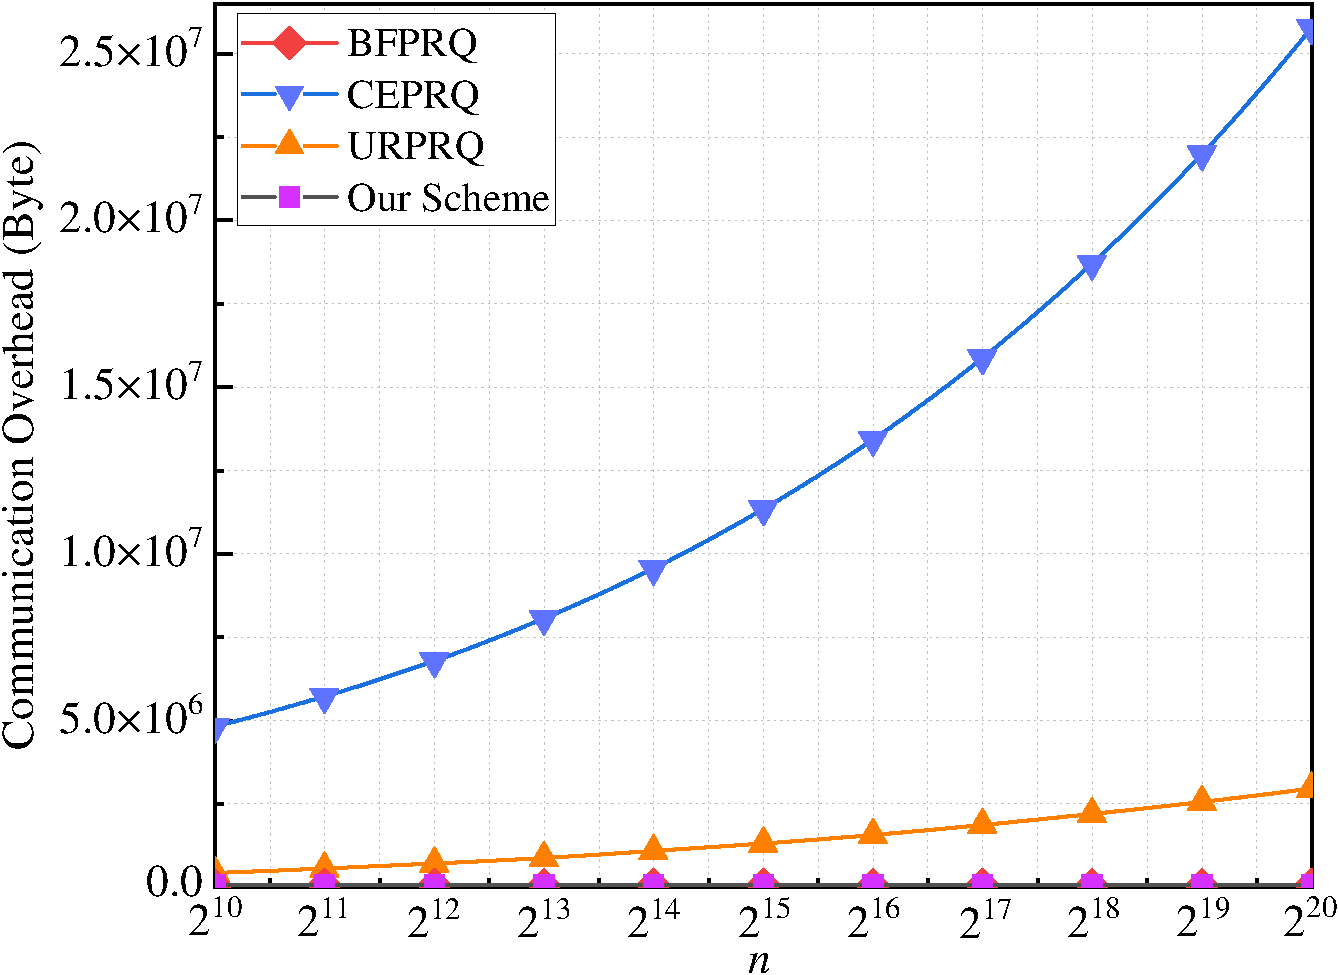
\includegraphics[width=1\textwidth]{commu_3n}\\
		\caption{Between \textcolor{blue}{the} edge server and \textcolor{blue}{IIoT} devices with varying $n$}\label{commu_3n}
	\end{subfigure}
	\quad
	\begin{subfigure}[t]{0.23\textwidth}
		\centering
		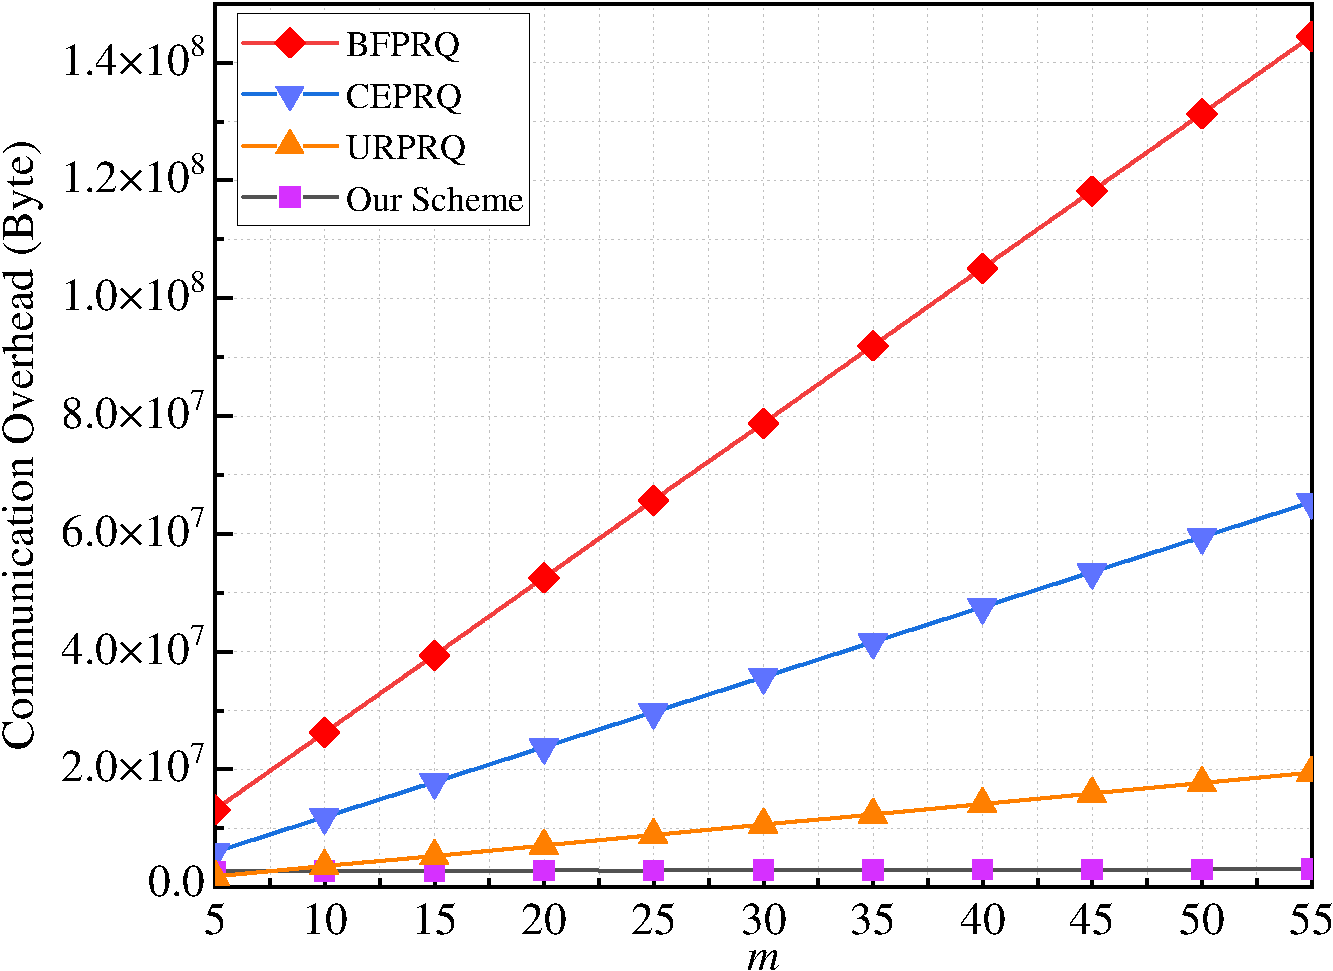
\includegraphics[width=1\textwidth]{commu_1m}\\
		\caption{Between \textcolor{blue}{the} edge server and \textcolor{blue}{the} query user with varying $m$}\label{commu_1m}	
	\end{subfigure}
	\quad
	\begin{subfigure}[t]{0.23\textwidth}
		\centering
		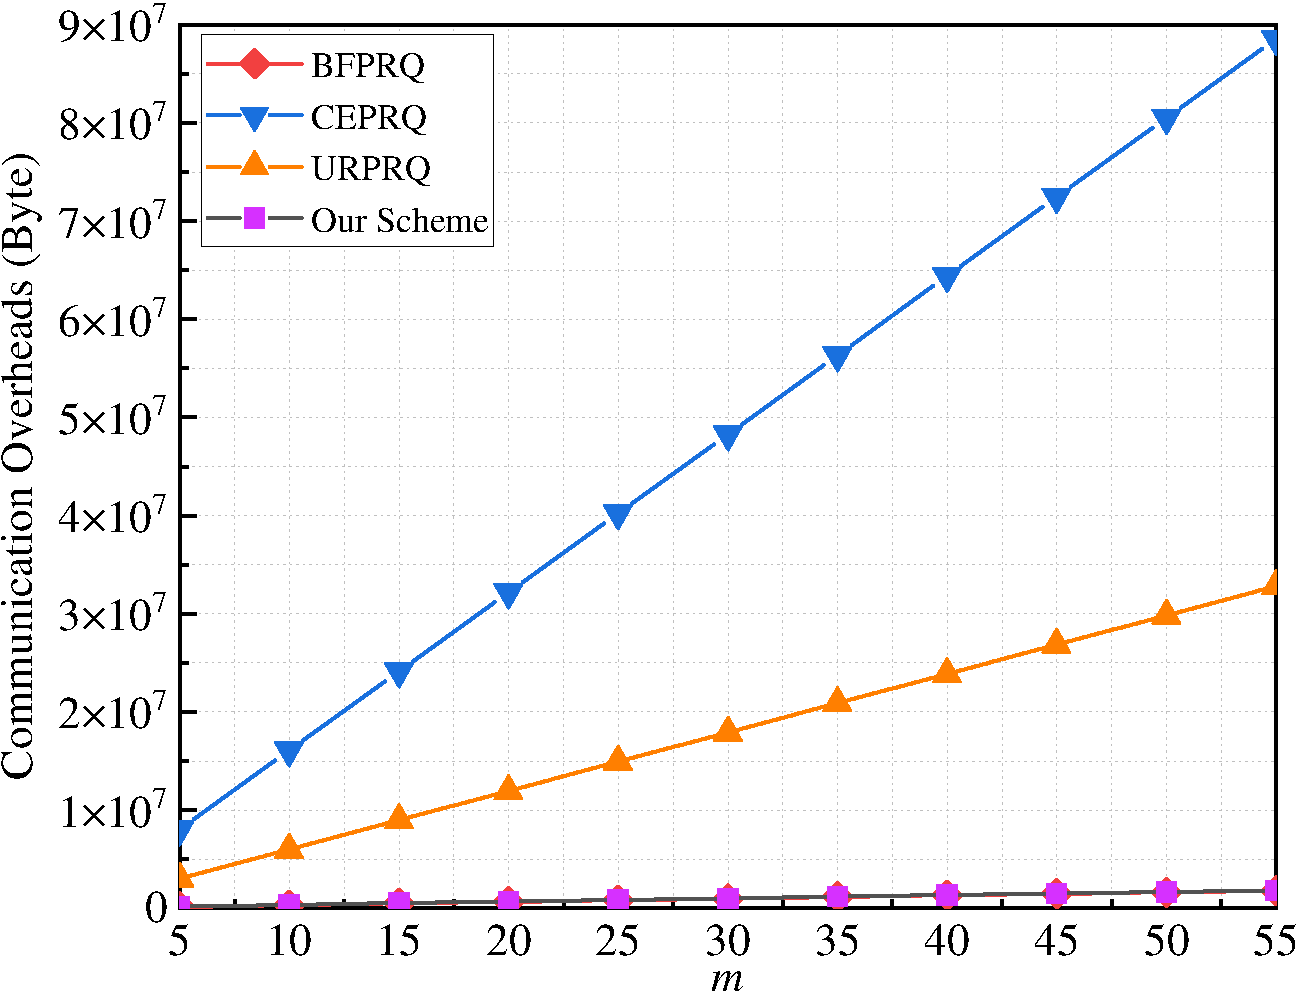
\includegraphics[width=1\textwidth]{commu_3m}\\
		\caption{Between \textcolor{blue}{the} edge server and \textcolor{blue}{IIoT} devices with varying $m$}\label{commu_3m}
	\end{subfigure}
	%\caption{Communication Overhead Comparison with varying $m$}\label{communication}
	\caption{Comparison of communication overhead }\label{communication}
\end{figure*}

\subsection{Communication overhead}
In this section, we compare the communication overhead of BFPRQ \cite{mahdikhani2020IoT}, CEPRQ \cite{hasan2020IoT}, URPRQ \cite{mahdikhani2020using} and Edge-PPMRQ. The communication overhead between \textcolor{blue}{the} edge server and \textcolor{blue}{the} query user includes both \textcolor{blue}{the} query request and \textcolor{blue}{the} query response. Besides, the communication overhead between \textcolor{blue}{the} edge server and \textcolor{blue}{IIoT} devices consists of \textcolor{blue}{the} data request and \textcolor{blue}{the} data response.

  For condition 1, we calculate the communication overhead of the four schemes between the edge server and the query user, and between the edge server and \textcolor{blue}{IIoT} devces, which are respectively shown in table \ref{commu_1_n} and table \ref{commu_2_n}.  In order to compare them more intuitively, Fig. \ref{commu_1n} and Fig. \ref{commu_3n} depict the communication overhead in condition 1. From the Fig. \ref{commu_1n}, we can see that the communication overhead between the edge server and the query user in Edge-PPMRQ keeps very low with $n$ varying from $2^{10}$ to $2^{20}$, while in BFPRQ \cite{mahdikhani2020IoT}, CEPRQ \cite{hasan2020IoT} and URPRQ \cite{mahdikhani2020using}, they grow rapidly. Fig. \ref{commu_3n} shows the communication overhead comparison between \textcolor{blue}{the} edge server and \textcolor{blue}{IIoT} devices, from which we can know that both Edge-PPMRQ and BFPRQ \cite{mahdikhani2020IoT} are equally efficient and perform significantly better than CEPRQ \cite{hasan2020IoT} and URPRQ \cite{mahdikhani2020using}.


 \iffalse
  (1) $m\cdot [b \cdot (n+|E_{paillier}|)+  |\lambda_i|)] + m \cdot |E_{paillier}| = 6 \cdot b\cdot(n+2048) + 16 \cdot 2048 +96= 16 \cdot n \cdot b + 32768 \cdot b + 32864$ (bits);   (2) $m \cdot [(2+\frac{2\cdot b^3+3\cdot b^2-11\cdot b}{6}) \cdot |E_{SHE}| + |\lambda_i|] +m \cdot |E_{SHE}| = 16\cdot[(2+\frac{2\cdot b^3+3\cdot b^2-11\cdot b}{6}) \cdot 160 \cdot (b+1) + 16\cdot 6]+ 16 \cdot 160 \cdot (b+1))= 2560/3  \cdot b^4 + 6400/3 \cdot b^3 + 10240/3 \cdot b^2 + 124160/3 \cdot b + 46176 $ (bits);  (3) $m \cdot [(b-1) \cdot (b+2) \cdot |E_{SHE}| + |\lambda_i|] + m \cdot |E_{SHE}| = 16 \cdot [(b-1) \cdot (b+2)\cdot |E_{SHE}|+ 6] + 16 \cdot |E_{SHE}| = 16 \cdot (b-1) \cdot (b+2) \cdot |E_{SHE} | = 2560 \cdot b^{3} + 2560 \cdot b^{2} + 96$ (bits).  (4) $b\cdot (n +m  \cdot |E_{OU}|) + m \cdot |\lambda_i| + m \cdot |E_{OU}| = b\cdot (n + 16 \cdot 1536) + 16 \cdot 1536 + 16 \cdot 6 =b \cdot n + 24576 \cdot b + 24672$ (bits); ,respectively, where $b=\rm{log}_2{n}$. Note that, $m$ is the number of dimensions in the query request. $|E_{paillier}|, |E_{SHE}|, |E_{OU}|$ and $|H|$ are the ciphertext length of paillier, SHE, OU and SHA-256, respectively.
\fi


    For condition 2, we also analyze the communication overhead of the four schemes between the edge server and \textcolor{blue}{the} query user, and between the edge server and \textcolor{blue}{IIoT} \textcolor{blue}{devices}, which are respectively shown in table \ref{commu_1_m} and table \ref{commu_2_m}. Similarly, Fig. \ref{commu_1m} and Fig. \ref{commu_3m} intuitively present the communication overhead of the four schemes in condition 2. From Fig. \ref{commu_1m}, the communication overhead between the edge server and the query user of the four schemes all show a linear growth trend, but the communication cost curve of Edge-PPMRQ is almost flat with \textcolor{blue}{$m$ varying} from $5$ to $55$, while the slopes of other schemes, BFPRQ \cite{mahdikhani2020IoT}, CEPRQ \cite{hasan2020IoT} and URPRQ \cite{mahdikhani2020using}, are much greater than that of Edge-PPMRQ. The reason is that Edge-PPMRQ achieves multi-dimensional range query by a query request, which saves a large number of communication \textcolor{blue}{costs} for \textcolor{blue}{multi-dimensional} query range. Fig. \ref{commu_3m} depicts the communication overhead between the edge server and \textcolor{blue}{IIoT} devices. From the figure, we find that the communication overhead in both Edge-PPMRQ and BFPRQ \cite{mahdikhani2020IoT} keeps efficient, but the communication \textcolor{blue}{costs} of CEPRQ \cite{hasan2020IoT} and URPRQ \cite{mahdikhani2020using} are almost $8$ times and $50$ times of that in Edge-PPMRQ, respectively. This is because in CEPRQ \cite{hasan2020IoT} and URPRQ \cite{mahdikhani2020using}, \textcolor{blue}{IIoT} devices not only receive the query request forwarded by the edge server, but also send ciphertext response back, which \textcolor{blue}{results} in a \textcolor{blue}{large amount of} communication overhead, while \textcolor{blue}{IIoT} devices of Edge-PPMRQ and BFPRQ \cite{mahdikhani2020IoT} only send keyed hash values $h( g^{ab} \| d_k)$ and dimension index $\lambda_i$ to the edge server, which are far shorter than ciphertext.

%(1) $m\cdot b \times (n+|E_{paillier}|)+m \times |E_{paillier}|+ m  \times |\lambda_i| = m \times 20 \times(2^{20} + 2048) + m \times 2048 + m \times 6 = 21014534 \cdot m $ (bits);
%  (2) $m\times((2+\frac{2\cdot b^3+3 \cdot b^2-11 \cdot b}{6})\times|E_{SHE}|)+m \times |E_{SHE}|+ m \times |\lambda_i|=m \times((2+\frac{2\cdot 20^3+3\cdot 20^2-11\cdot 20}{6}) \times(160\times (20+1))) + m \times 160\times (20+1)+ m \times 6 = 9518886 \cdot m $ (bits);
% (3) $b\times (n +m\times|E_{OU}|) + m \times |E_{OU}| + m \times |\lambda_i| = 20 \times (2^{20} + m \times 1536 ) + m \times 6 =  30726 \cdot m + 20971520$ (bits);
% (4) $ m \times (b-1) \times (b+2) \times |E_{SHE}| = 418 \times m \times |E_{SHE}|$ (bits), respectively.

   \begin{table*}
 	\caption{Communication overhead between the edge server and the query user}\label{commu_1_m}
 	\begin{center}
 		\begin{tabular}{ l  l  l  l }
 			\hline
 			Schemes  & Query request (bits)& Query result (bits)& Total overhead (bits) \\ \hline
 			BFPRQ    & $m\cdot [b \cdot (n+|E_{paillier}|)+  |\lambda_i|)]$  & $m \cdot (|E_{paillier}| + |\lambda_i|)$ & $21014534 \cdot m $ \\
 			CEPRQ       & $m \cdot [(2+\frac{2\cdot b^3+3\cdot b^2-11\cdot b}{6}) \cdot |E_{SHE}| + |\lambda_i|]$ & $m \cdot (|E_{SHE}| + |\lambda_i|) $ & $ 9518886 \cdot m $  \\
 			URPRQ       & $m \cdot [(b-1) \cdot (b+2) \cdot |E_{SHE}| + |\lambda_i|]$ & $m \cdot (|E_{SHE}|+ |\lambda_i|)$ & $858124 \cdot m$ \\
 			Edge-PPMRQ  & $b\cdot (n +m  \cdot |E_{OU}|) + m \cdot |\lambda_i| $     &  $m \cdot (|E_{OU}|+ |\lambda_i|)$  &  $30726 \cdot m + 20971520$ \\ \hline
 		\end{tabular}
 	\end{center}
 \end{table*}

\setlength{\floatsep}{1pt}

  \begin{table*}[htbp]
 	\caption{Communication overhead between the edge server and the \textcolor{blue}{IIoT} devices}\label{commu_2_m}
 	\begin{center}
 		\begin{tabular}{ l  l  l  l }
 			\hline
 			Schemes  & Data request (bits)& Data response (bits)& Total overhead (bits) \\ \hline
 			BFPRQ    & $m \cdot |\lambda_i|$  & $m \cdot N \cdot (|H| + |\lambda_i|)$ & $262000 \cdot m$ \\
 			CEPRQ       & $m \cdot [(2+\frac{2\cdot b^3+3\cdot b^2-11\cdot b}{6}) \cdot |E_{SHE}| + |\lambda_i|]$ & $m \cdot N \cdot  (|E_{SHE}| + |\lambda_i|)$ & $ 12881520 \cdot m $  \\
 			URPRQ       & $m \cdot [(b-1) \cdot (b+2) \cdot |E_{SHE}| + |\lambda_i|]$ & $m \cdot N \cdot  (|E_{SHE}| + |\lambda_i|)$ & $2048000 \cdot m $ \\
 			Edge-PPMRQ  & $m \cdot |\lambda_i|$   &  $m \cdot N \cdot (|H| + |\lambda_i|)$  & $262000 \cdot m$ \\ \hline
 		\end{tabular}
 	\end{center}
 \end{table*}

\vspace{-0cm}

%  (1) $m \cdot N \cdot (|\lambda_i| + |H_{SHA3-256}|)= 262000 \cdot m$ (bits);
%  (2) $m\times((2+\frac{2\cdot b^3+3\cdot b^2-11\cdot b}{6}) \times |E_{SHE}|) +N \times (|\lambda_i| + |E_{SHE}|) = m\times((2+\frac{2\cdot 20^3+3\cdot 20^2-11\cdot 20}{6}) \times 160 \times (20 + 1))  + 1000 \times m \times ( 6 + 160(20+1)) = 12881520 \cdot m $ (bits);
%  (3)  $m \times N \times |E_{SHE}|= 1000 \cdot m \cdot |E_{SHE}|=2048000 \cdot m $
%  (4) $m \times N \times (|\lambda_i| + |H_{SHA3-256}|)= 262000 \cdot m$ (bits), respectively.



  Based on the above comparisons, we can conclude that Edge-PPMRQ is remarkably communication-efficient.



\begin{figure*}
	\setlength{\abovecaptionskip}{0.cm}	
	\centering
	\begin{subfigure}[t]{0.3\textwidth}
		\centering	
		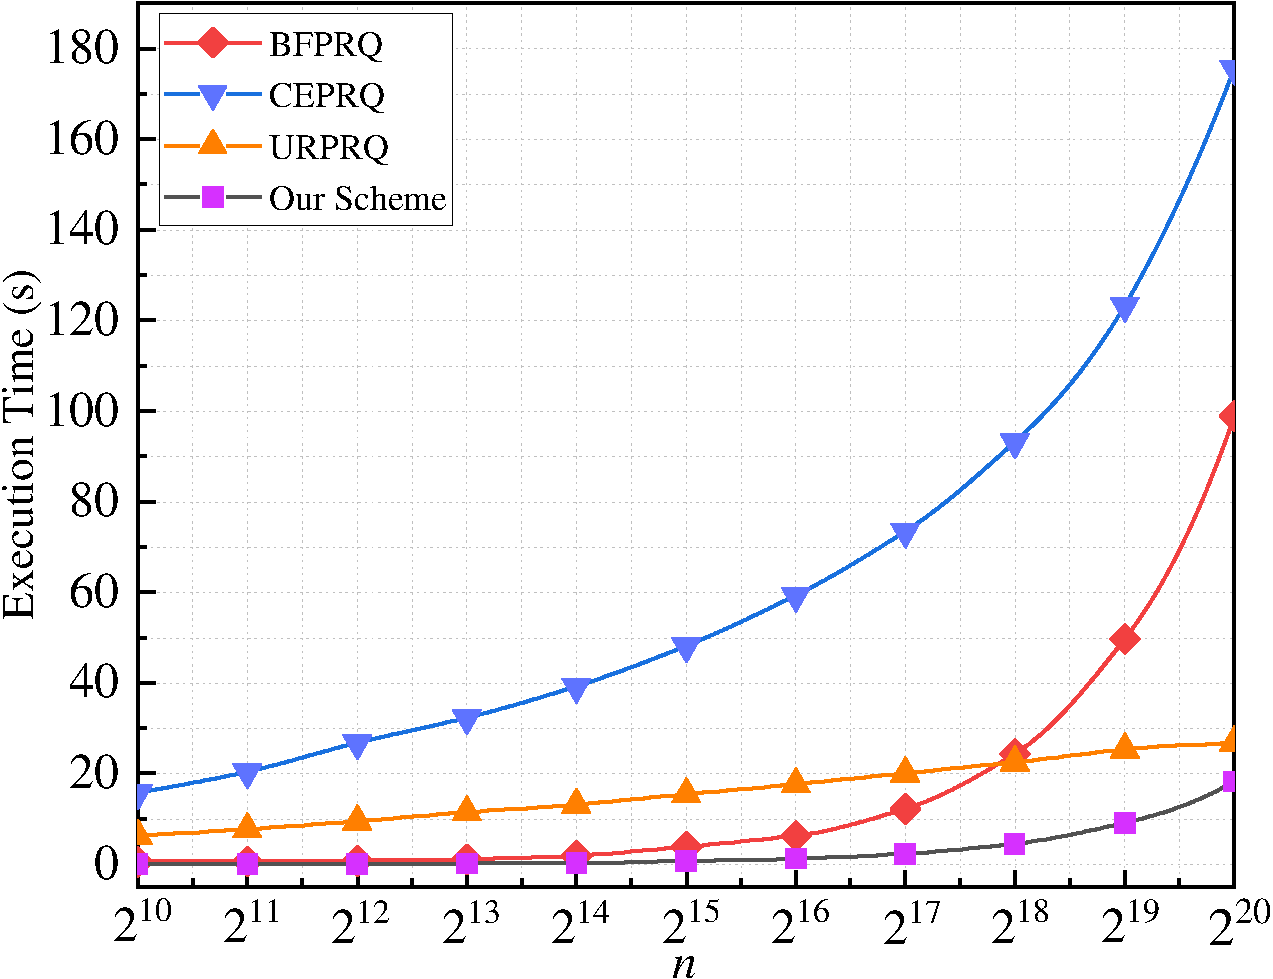
\includegraphics[width=1\textwidth]{com_1n}\\
		\caption{Time cost of user side}
		\label{com_1n}
	\end{subfigure}
	\quad
	\begin{subfigure}[t]{0.3\textwidth}
		\centering
		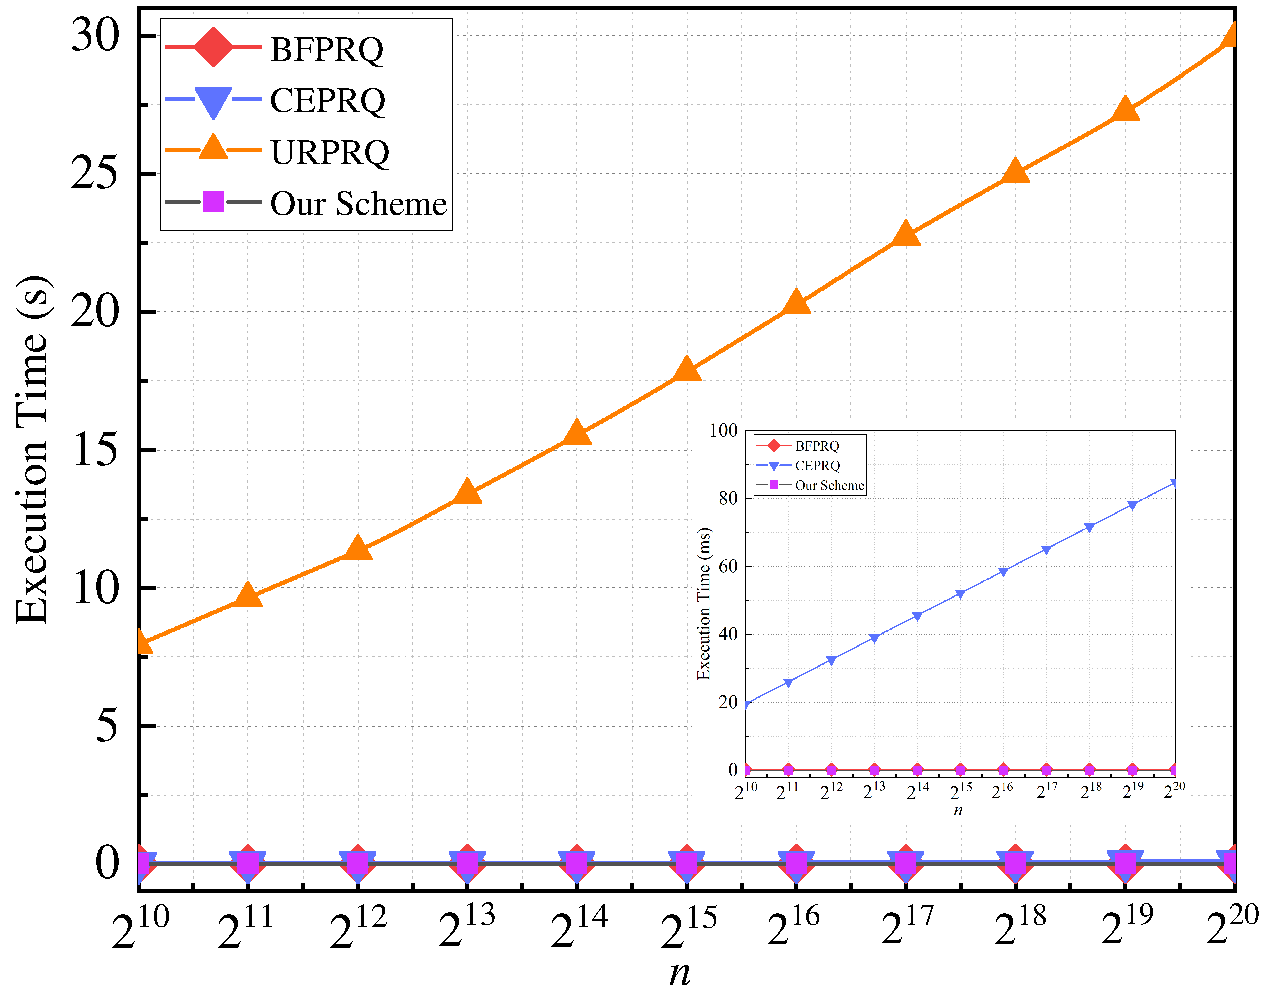
\includegraphics[width=1\textwidth]{com_2n_12}\\
		\caption{Time cost of \textcolor{blue}{IIoT} side}
		\label{com_2n}
	\end{subfigure}
	\quad
	\begin{subfigure}[t]{0.3\textwidth}
		\centering
		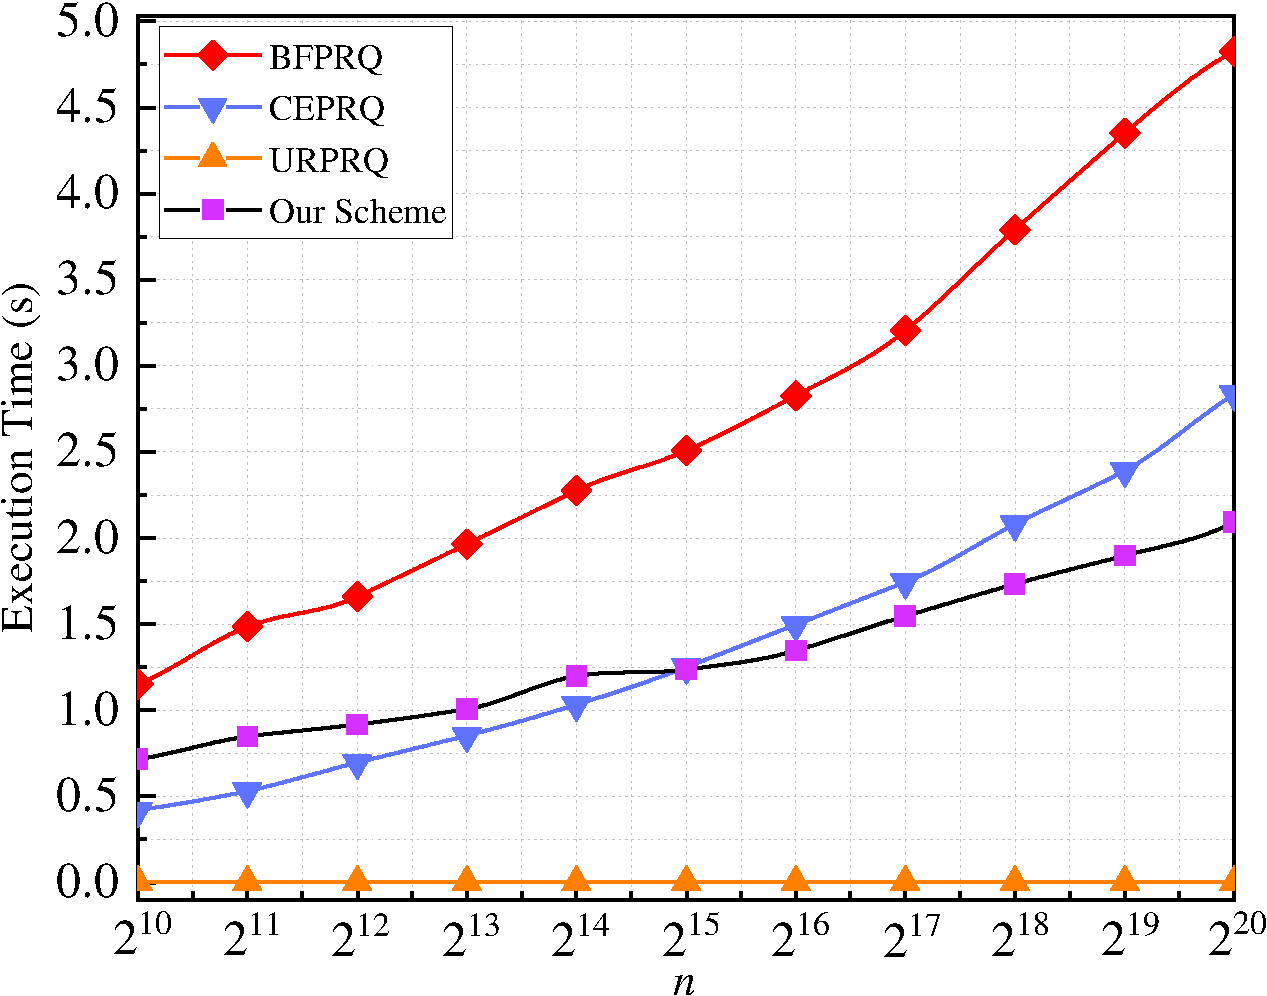
\includegraphics[width=1\textwidth]{com_3n}\\
		\caption{Time cost of edge server side}
		\label{com_3n}
	\end{subfigure}
	\caption{Computational time cost comparison with varying $n$}\label{computation_n}
\end{figure*}

\begin{figure*}%[htbp]	
	\centering
	\begin{subfigure}[t]{0.3\textwidth}
		\centering
		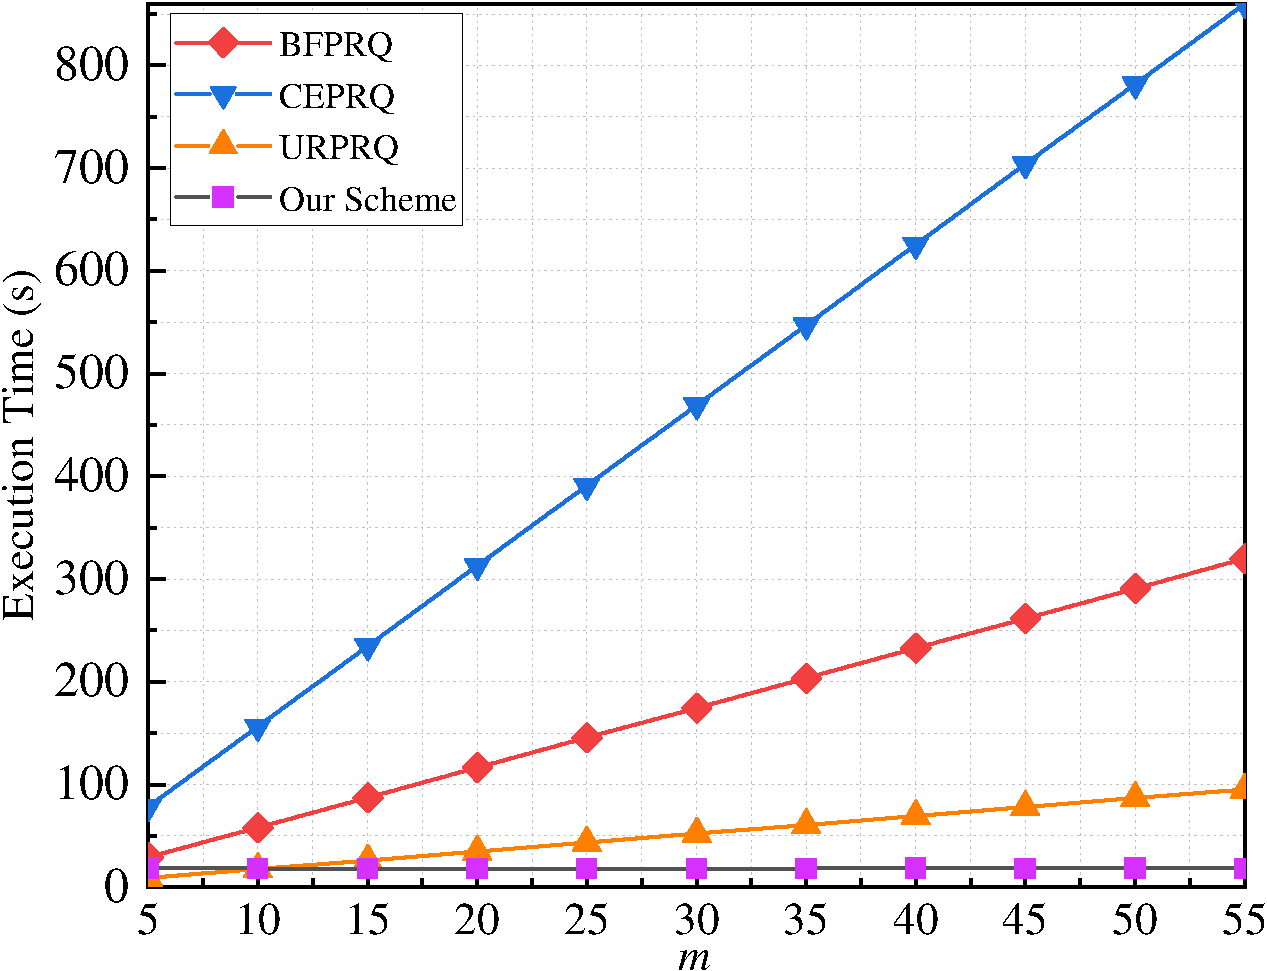
\includegraphics[width=1\textwidth]{com_1m}\\
		\caption{Time cost of user side}\label{com_1m}	
	\end{subfigure}
	\quad
	\begin{subfigure}[t]{0.3\textwidth}
		\centering
		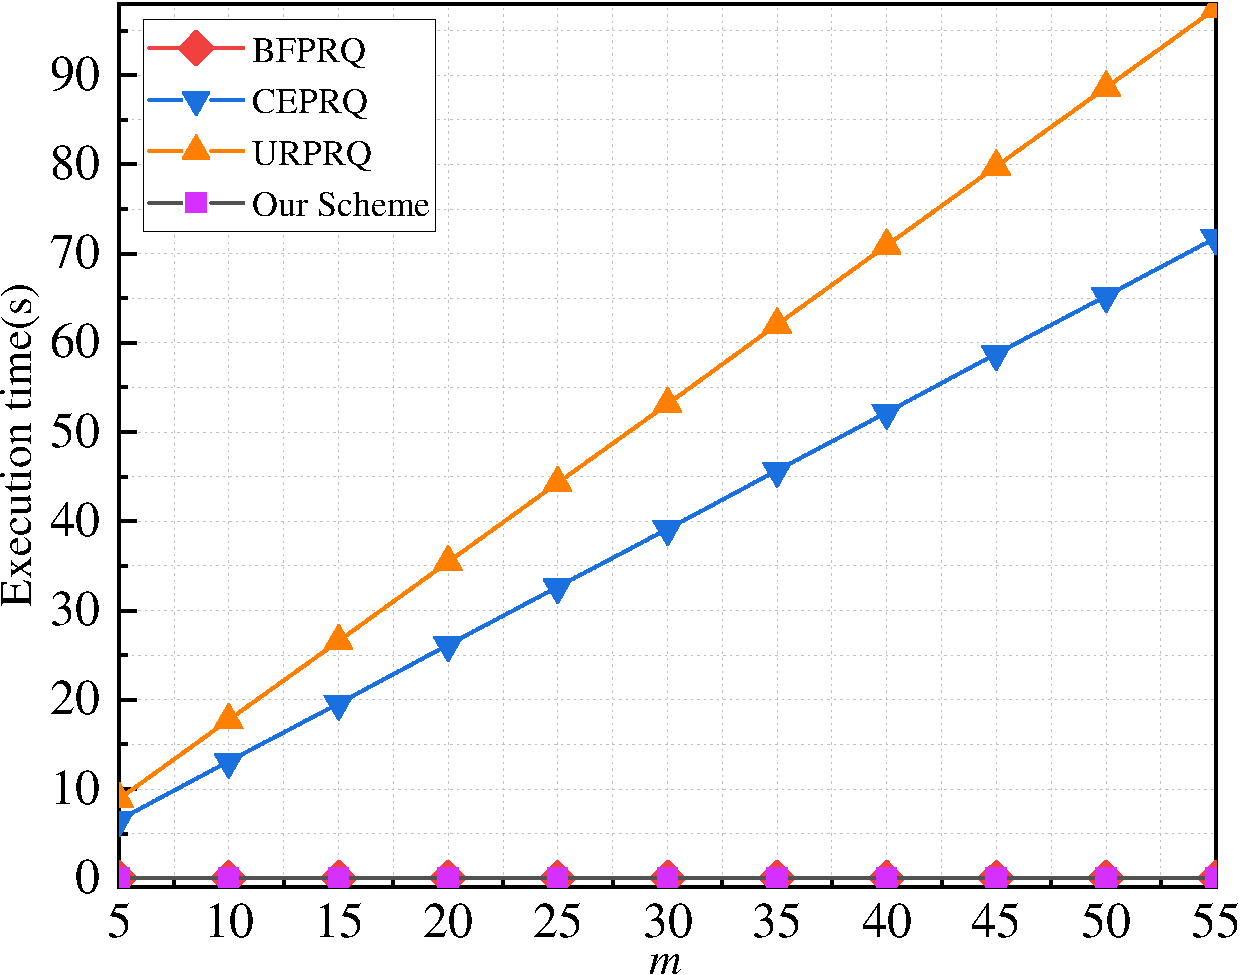
\includegraphics[width=1\textwidth]{com_2m}\\
		\caption{Time cost of \textcolor{blue}{IIoT} side}\label{com_2m}
	\end{subfigure}
	\quad
	\begin{subfigure}[t]{0.3\textwidth}
		\centering
		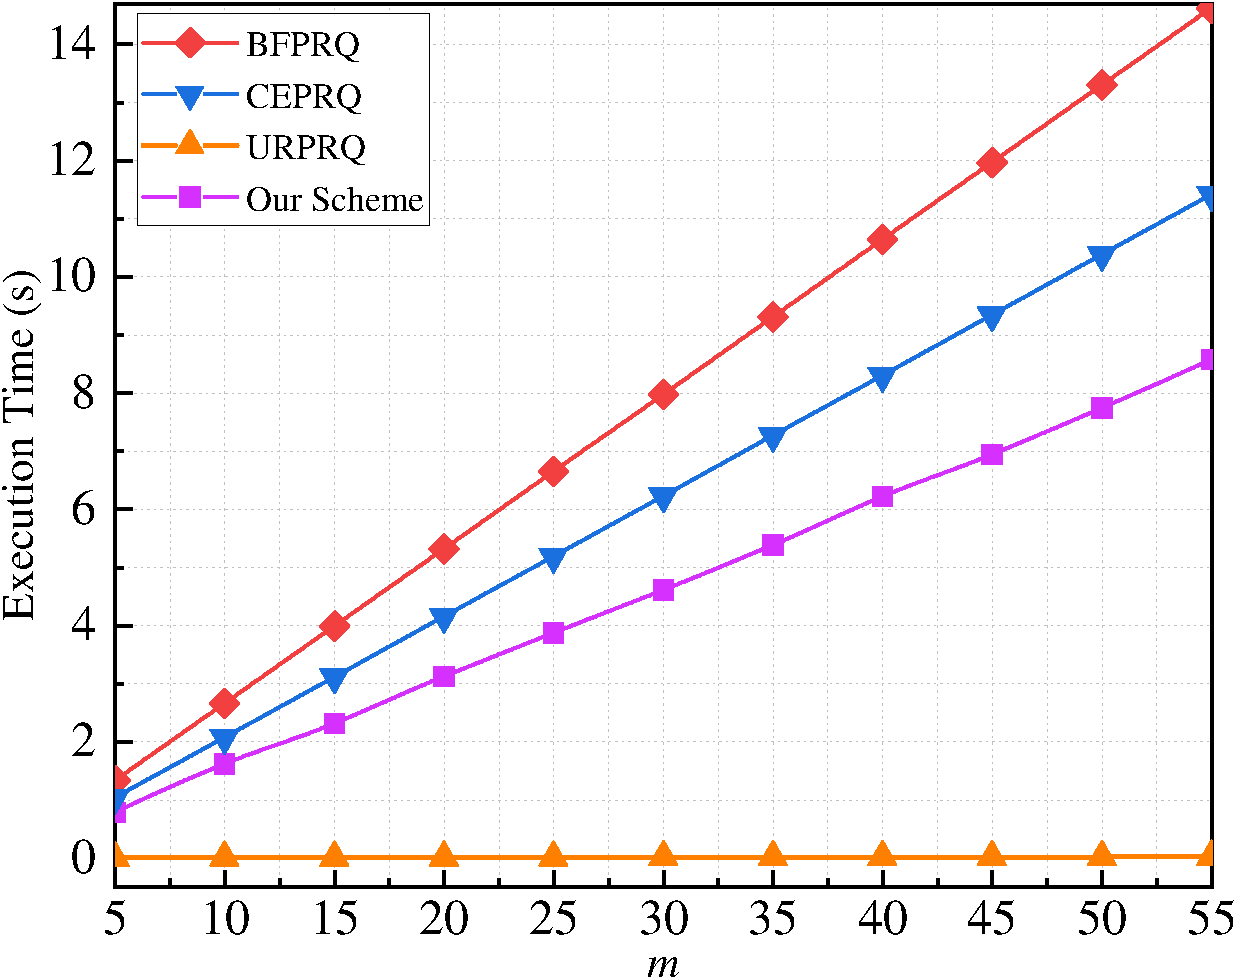
\includegraphics[width=1\textwidth]{com_3m}\\
		\caption{Time cost of edge server side}\label{com_3m}
	\end{subfigure}
	\caption{Computational time cost comparison with varAying $m$}\label{computation_m}
\end{figure*}


%Paillier?OU????????
\vspace{-0cm}
\begin{table*}\centering
	
	\caption{\textcolor{blue}{Comparison between Paillier and OU}}
	
	\begin{tabular*}{15cm}{p{3.0cm}cccc}
		
		\hline
		\textcolor{blue}{Algorithm/Operations} & \textcolor{blue}{Encryption(ms)} & \textcolor{blue}{Decryption(ms)} & \textcolor{blue}{Homomorphic Addition(ms)} & \textcolor{blue}{Scalar Multiplication(ms)} \\
		\hline
		\textcolor{blue}{Paillier}            & $12.4$     & $12.4$    & $0.023$    & $0.096$ \\
		\textcolor{blue}{Okamoto Uchiyama}    & $10.5$     & $1.8$  & $0.012$  & $0.062$ \\\hline
	\end{tabular*}
	\label{encryption}
\end{table*}



\begin{table*}\centering
	
	\caption{\textcolor{blue}{Functional comparison}}
	
	\begin{tabular*}{14.7cm}{p{6.5cm}cccc}
		
		\hline
		Schemes & Edge-PPMRQ & BFPRQ \cite{mahdikhani2020IoT} & CEPRQ \cite{hasan2020IoT} & URPRQ \cite{mahdikhani2020using} \\
		\hline
		Multi-dimension             & $\surd$     & $\times$    & $\times$    & $\times$ \\
		Discotinuous range         & $\surd$     & $\surd$  & $\times$  & $\surd$ \\
		Arbitrary boundary range            & $\surd$     & $\surd$  & $\times$  & $\surd$ \\
		\textcolor{blue}{\textcolor{blue}{Counting} function} & $\surd$ & $\surd$  & $\surd$  & $\surd$ \\
		\textcolor{blue}{Sum function} & $\times$ & $\times$ & $\surd$ & $\surd$\\
		\textcolor{blue}{Suitability for IIoT applications} & $\surd$ & $\surd$  & $\times$ & $\times$ \\
		\iffalse
		\textcolor{blue}{Communication costs between \textcolor{blue}{IIoT} and edge server(Bytes)} &  $1.80\times10^6$  &   $1.80\times10^6$    & $8.86\times 10^7$   & $1.41\times 10^7$ \\	
		\textcolor{blue}{Communication costs between query user and edge server(Bytes)} & $2.83\times 10^6$      & $1.44\times 10^8$      & $6.54 \times 10^7$      & $5.90 \times 10^6$ \\	
		\textcolor{blue}{computational cost in IIoT(ms)} &    0.01323     & 0.73536         & 71748.1115	      & 97439.4401 \\
		\textcolor{blue}{computational cost in edge server(ms)} & 8575.7 & 14624.0      & 11415.7    & 21.9 \\
		\textcolor{blue}{computational cost in query user(ms)} &  18218.7      & 319675.3      & 859984.1 & 95028.4 \\
		\fi
		\hline
	\end{tabular*}
	\label{comprehensive comparison}
	
\end{table*}

\subsection{Computational cost}
In this section, we compare the execution time \textcolor{blue}{of} the query user, \textcolor{blue}{IIoT} devices and the edge server with varying $n$ and $m$, \textcolor{blue}{respectively}, and the experiment comparison results are taken from the average value of 10 times simulations. \textcolor{blue}{Our scheme uses \textcolor{blue}{OU cryptosystem}, while some of the compared schemes utilize Paillier cryptosystem. Therefore, we give the time cost comparison between Paillier and OU in Table \ref{encryption}. From the table, we can see that \textcolor{blue}{OU cryptosystem} is more efficient than Paillier cryptosystem.} 


Fig. \ref{computation_n} shows the average computational time of BFPRQ \cite{mahdikhani2020IoT}, CEPRQ \cite{hasan2020IoT}, URPRQ \cite{mahdikhani2020using} and Edge-PPMRQ in condition 1. Specifically, Fig. \ref{com_1n} illustrates the execution time of the query user, including user query request generation and response recovery. From the figure, we can see that Edge-PPMRQ is really efficient, while the execution time of BFPRQ \cite{mahdikhani2020IoT}, CEPRQ \cite{hasan2020IoT} and URPRQ \cite{mahdikhani2020using} increases rapidly with $n$ varying from $2^{10}$ to $2^{20}$. For example, when $n=2^{20}$, the execution time of BFPRQ \cite{mahdikhani2020IoT} and CEPRQ \cite{hasan2020IoT} are $4$ times and $7$ times of that in Edge-PPMRQ, respectively. URPRQ \cite{mahdikhani2020using} also obviously consumes more execution time than Edge-PPMRQ. \textcolor{blue}{The reason for the excellent performance of Edge-PPMRQ is that Edge-PPMRQ maps multiple query ranges into a \textcolor{blue}{group of bloom filters}, so that the range query requests for multiple dimensions can be realized by only one query request, while in other schemes, the query user has to send multiple query requests to achieve the same purpose}. Fig. \ref{com_2n} \textcolor{blue}{illustrates} the execution time \textcolor{blue}{of} \textcolor{blue}{IIoT} devices. \textcolor{blue}{It} shows that in URPRQ \cite{mahdikhani2020using}, \textcolor{blue}{IIoT} devices undertake \textcolor{blue}{considerable computational costs}, while the execution time of BFPRQ \cite{mahdikhani2020IoT}, CEPRQ \cite{hasan2020IoT} and Edge-PPMRQ is negligible. Furthermore, a sub-figure in Fig. \ref{com_2n} is given to better illustrate the comparison among BFPRQ \cite{mahdikhani2020IoT}, CEPRQ \cite{hasan2020IoT} and Edge-PPMRQ. From the sub-figure, we can see that the execution time of CEPRQ \cite{hasan2020IoT} also grows more rapidly than \textcolor{blue}{that of} Edge-PPMRQ and BFPRQ \cite{mahdikhani2020IoT} \textcolor{blue}{increases}. \textcolor{blue}{The reason for the result is that in CEPRQ \cite{hasan2020IoT} and URPRQ \cite{mahdikhani2020using}, \textcolor{blue}{IIoT} devices perform a lot of time-consuming operations, i.e., homomorphic addition and homomorphic xor, while in Edge-PPMRQ and BFPRQ \cite{mahdikhani2020IoT}, \textcolor{blue}{IIoT} devices only compute the keyed hash value, which is much more efficient than homomorphic operations.} Fig. \ref{com_3n} indicates the execution time \textcolor{blue}{of} the edge server. From the figure, we can observe that Edge-PPMRQ, CEPRQ \cite{hasan2020IoT} and URPRQ \cite{mahdikhani2020using} are more efficient than BFPRQ \cite{mahdikhani2020IoT}, and  Edge-PPMRQ performs better than CEPRQ \cite{hasan2020IoT} when $n$ is bigger than $2^{15}$. Although the computational cost of the edge server in URPRQ \cite{mahdikhani2020using} \textcolor{blue}{keeps} very low, it is at the cost of a large amount of computational overhead for \textcolor{blue}{IIoT} devices  according to Fig. \ref{com_2n}.



Fig. \ref{computation_m} depicts the average computational time of BFPRQ \cite{mahdikhani2020IoT}, CEPRQ \cite{hasan2020IoT}, URPRQ \cite{mahdikhani2020using} and Edge-PPMRQ in condition 2. Specifically, Fig. \ref{com_1m} shows the execution time \textcolor{blue}{of} the query user, including two parts, i.e., user query request generation and response recovery. We can find that Edge-PPMRQ costs nearly constant execution time, which is apparently efficient than BFPRQ \cite{mahdikhani2020IoT}, CEPRQ \cite{hasan2020IoT} and URPRQ \cite{mahdikhani2020using}. This is because the query user in Edge-PPMRQ performs less homomorphic operations than BFPRQ \cite{mahdikhani2020IoT}, CEPRQ \cite{hasan2020IoT} and URPRQ \cite{mahdikhani2020using}. Fig. \ref{com_2m} depicts \textcolor{blue}{IIoT} devices' data response time, which shows that both Edge-PPMRQ and BFPRQ \cite{mahdikhani2020IoT} are more efficient than CEPRQ \cite{hasan2020IoT} and URPRQ \cite{mahdikhani2020using}. The reason is that \textcolor{blue}{IIoT} devices in Edge-PPMRQ and BFPRQ \cite{mahdikhani2020IoT} only need compute keyed hash values $H( g^{ab} \| d_i)$, while both in CEPRQ \cite{hasan2020IoT} and URPRQ \cite{mahdikhani2020using}, \textcolor{blue}{IIoT} devices need perform \textcolor{blue}{a large number of} homomorphic multiplication operations. Fig. \ref{com_3m} presents the data aggregation time cost \textcolor{blue}{of} the edge server, \textcolor{blue}{which shows that} Edge-PPMRQ performs better than BFPRQ \cite{mahdikhani2020IoT} and CEPRQ \cite{hasan2020IoT} since in Edge-PPMRQ, the number of homomorphic operations are less than that of BFPRQ \cite{mahdikhani2020IoT} and CEPRQ \cite{hasan2020IoT}. Obviously, URPRQ \cite{mahdikhani2020using} consumes the \textcolor{blue}{least} computational time. The reason is that the most computational \textcolor{blue}{cost is} afforded by \textcolor{blue}{IIoT} devices, and the edge server only performs homomorphic addition operations.



\subsection{\textcolor{blue}{Functional} comparison}
Based on above \textcolor{blue}{introduction} and analysis, a \textcolor{blue}{functional} comparison of Edge-PPMRQ and related schemes is given in table \ref{comprehensive comparison}.

From a functional point of view, Edge-PPMRQ supports the functions of \textcolor{blue}{multi-dimensional}, discontinuous and arbitrary-boundary range query, while BFPRQ \cite{mahdikhani2020IoT}, CEPRQ \cite{hasan2020IoT} and URPRQ  \cite{mahdikhani2020using} cannot support \textcolor{blue}{multi-dimensional} range query. Additionally, CEPRQ \cite{hasan2020IoT} also cannot support discontinuous \textcolor{blue}{range} query \textcolor{blue}{or} arbitrary-boundary range query. \textcolor{blue}{ Moreover, with respect to query functions, all the 4 schemes support the \textcolor{blue}{Counting} function, i.e., the query user can get the number of the sensed data located in the query range. Besides, CEPRQ and URPRQ can also achieve sum function, i.e., the query user can obtain the sum of the sensed data within the query range.}

From a \textcolor{blue}{real application perspective, edge/fog computing is introduced for decreasing the load of \textcolor{blue}{IIoT} devices and reducing the delay of service. Therefore,}
in edge/fog-supported IIoT \textcolor{blue}{applications}, \textcolor{blue}{some tasks of IIoT devices can be migrated to edge server/fog node}, 
\iffalse
 Consequently, the communication overhead and computational cost of IIoT devices can be greatly reduced,
 \fi
 which not only remarkably extends the life period of IIoT devices, but also \textcolor{blue}{provides} nearly real-time service. According to the comparison in \textcolor{blue}{the Fig. \ref{communication}, Fig. \ref{computation_n} and Fig. \ref{computation_m}, the costs of \textcolor{blue}{IIoT} devices in Edge-PPMRQ and BFPRQ \cite{mahdikhani2020IoT}} \textcolor{blue}{evidently keeps very low}, while in CEPRQ \cite{hasan2020IoT} and URPRQ \cite{mahdikhani2020using}, \textcolor{blue}{IIoT} devices \textcolor{blue}{process a larger proportion of communication and computational tasks. Therefore, Edge-PPMRQ and BFPRQ \cite{mahdikhani2020IoT} are considerably suitable for IIoT applications.}

\iffalse
 Although BFPRQ \cite{mahdikhani2020IoT} has \textcolor{blue}{relatively} low communication overhead between \textcolor{blue}{IIoT} devices and the edge server and low computational cost in \textcolor{blue}{IIoT} devices, its computational cost in edge server side is high. CEPRQ \cite{hasan2020IoT} has middle communication overhead between \textcolor{blue}{IIoT} devices and the edge server, and computational cost in the edge server, but it consumes high execution time in \textcolor{blue}{IIoT} devices. Moreover, URPRQ \cite{mahdikhani2020using} not only has high communication overhead between \textcolor{blue}{IIoT} and edge server, but also consumes high computational cost in \textcolor{blue}{IIoT} devices. Although URPRQ \cite{mahdikhani2020using} has lowest computational cost in fog node, it is at the cost of high computational load in \textcolor{blue}{IIoT} devices. Therefore, it is not suitable for edge/fog-supported \textcolor{blue}{IIoT} applications, in which the \textcolor{blue}{IIoT} devices own limited resource.
\fi

In a word, Edge-PPMRQ not only is functionally powerful for \textcolor{blue}{multi-dimensional}, discontinuous and arbitrary boundary range queries, but also \textcolor{blue}{is significantly suitable} for I\textcolor{blue}{IIoT} applications.

\iffalse
From a performance perspective, in edge/fog-supported \textcolor{blue}{IIoT} application, the most important mission of edge server/fog node is to reduce the burden of \textcolor{blue}{IIoT} devices, and the most tasks of devices can be migrated to edge server/fog node. As a result, the communication overhead and computational cost of \textcolor{blue}{IIoT} side can be greatly reduced. This not only remarkably extends the life period of \textcolor{blue}{IIoT} devices, but also achieves nearly real-time service. According to the comparison in the table \ref{comprehensive comparison}, Edge-PPMRQ and BFPRQ \cite{mahdikhani2020IoT} achieve the purpose well, while in CEPRQ \cite{hasan2020IoT} and URPRQ \cite{mahdikhani2020using}, \textcolor{blue}{IIoT} side takes the most communication and computational tasks. Although BFPRQ \cite{mahdikhani2020IoT} has high computational cost in edge server side and CEPRQ \cite{hasan2020IoT} consumes high execution time in IoT side. Moreover, URPRQ \cite{mahdikhani2020using} not only has high communication overhead between \textcolor{blue}{IIoT} and edge server, but also consumes high computational cost in \textcolor{blue}{IIoT} side. Although URPRQ \cite{mahdikhani2020using} has lowest computational cost in fog node, it is at the cost of high computational load in \textcolor{blue}{IIoT} side, therefore, .
\fi

\iffalse
More importantly, in edge-supported IIoT, fog node and edge server are introduced to employ the most communication and computational cost and support nearly real-time data process. As a result, the communication overhead and computational cost of IIoT side can be greatly reduced, which can remarkably extend the life period of IIoT side. According to the comparison in the table, Edge-PPMRQ and BFPRQ \cite{mahdikhani2020IoT} achieve the purpose well, while in CEPRQ \cite{hasan2020IoT} and URPRQ \cite{mahdikhani2020using}, IIoT side takes the most communication and computational tasks. So, we can conclude that Edge-PPMRQ is the comprehensively best.


Furthermore, in edge/fog-supported IIoT application, the most important mission of edge server/fog node is to reduce the burden of IIoT devices, and the most tasks of devices can be migrated to edge server/fog node. As a result, the communication overhead and computational cost of IIoT side can be greatly reduced. This not only remarkably extends the life period of IIoT devices, but also achieves nearly real-time service. According to the comparison in the table, Edge-PPMRQ and BFPRQ \cite{mahdikhani2020IoT} achieve the purpose well, while in CEPRQ \cite{hasan2020IoT} and URPRQ \cite{mahdikhani2020using}, IIoT side takes the most communication and computational tasks. Although URPRQ \cite{mahdikhani2020using} has lowest computational cost in fog node, it is at the cost of high computational load in IIoT side, the . So, we can conclude that Edge-PPMRQ is the comprehensively best.
\fi



\section{Conclusion and future work}
 Based on our proposed \textcolor{blue}{range} division algorithm, this paper has designed a privacy-preserving multi-dimensional range query scheme for edge-supported IIoT. \textcolor{blue}{The scheme} achieves the function of multi-dimensional range query, i.e. a user can query different types of data at once, which is very suitable for the real application of IIoT environment. Meanwhile, it also supports the continuous, discontinuous and \textcolor{blue}{arbitrary-boundary} range queries. The security analysis proves that Edge-PPMRQ is privacy-preserving, i.e. the query ranges and \textcolor{blue}{the} query results cannot be revealed by any entities except the query user, and the sensed data of each IIoT device cannot be recovered by other parties. Furthermore, a large number of experiments are conducted to evaluate \textcolor{blue}{and compare} the performance of Edge-PPMRQ and other related work, and the results show that Edge-PPMRQ is really communication and computationally efficient. Comprehensively, Edge-PPMRQ achieves expected goals in aspects of functions, privacy preservation and efficiency. 
 
 In future work, we plan to study more efficient range query schemes for various functions, privacy requirements and multiple application scenarios, e.g., multi-user range query scheme.

\footnotesize
\bibliographystyle{IEEEtran}
\bibliography{IEEEabrv,references}
\vspace{12 pt}
\normalsize

\iffalse
\noindent\textbf{Xiong Li} received the Ph.D. degree in computer science and technology from the Beijing University of Posts and Telecommunications, Beijing, China, in 2012. He is currently an Associate Professor with the School of Computer Science and Engineering, Hunan University of Science and Technology, Xiangtan, China. He has authored over 100 referred papers. His current research interests include cryptography and information security. He was a recipient of the 2015 Journal of Network and Computer Applications Best Research Paper Award.\\

\noindent\textbf{Shanpeng Liu}
 is currently a M.S. candidate of Hunan University of Science and Technology, China. His research interests include cloud computing security and security protocols.\\

\noindent\textbf{Fan Wu} received the ME degree in computer software and theory from Xiamen University, Xiamen, China, in 2008. Now, he is an Associate Professor in Xiamen Institute of Technology. His current research interests include information security, internet protocols, and network management.\\

\noindent\textbf{Saru Kumari} received the Ph.D. degree in mathematics from Chaudhary Charan Singh University, Meerut, India, in 2012. She is currently an Assistant Professor in the
Department of Mathematics, Chaudhary Charan Singh University. Her current research interests include information security, digital authentication, and applied mathematics.\\

\noindent\textbf{Joel J.P.C. Rodrigues} (S01, M06, SM06) is a professor and senior researcher at the National Institute of Telecommunications (Inatel), Brazil and senior researcher at the Instituto de Telecomunica\c{c}\~oes, Portugal. Prof. Joel is the leader of the Internet of Things Research Group (Inatel), Director for Conference Development-IEEE ComSoc Board of Governors, and IEEE Distinguished Lecturer. He has authored or coauthored over 650 papers in refereed international journals and conferences, 3 books, and 2 patents. He had been awarded several Outstanding Leadership and Outstanding Service Awards by IEEE Communications Society and several best papers awards.




\vspace{-1cm}
\begin{IEEEbiography}[{\includegraphics[width=1in,height=1.25in,clip,keepaspectratio]{1.jpg}}]{Xiong Li}
received the Ph.D. degree in computer science and technology from the Beijing University of Posts and Telecommunications, Beijing, China, in 2012. He is currently an Associate Professor with the School of Computer Science and Engineering, Hunan University of Science and Technology, Xiangtan, China. He has authored over 100 referred papers. His current research interests include cryptography and information security. He was a recipient of the 2015 Journal of Network and Computer Applications Best Research Paper Award.
\end{IEEEbiography}

\vspace{-1.5cm}
\begin{IEEEbiography}[{\includegraphics[width=1in,height=1.25in,clip,keepaspectratio]{2.jpg}}]{Shanpeng Liu}
 is currently a M.S. candidate of Hunan University of Science and Technology, China. His research interests include cloud computing security and security protocols.
\end{IEEEbiography}
\vspace{-1.5cm}

\begin{IEEEbiography}[{\includegraphics[width=1in,height=1.25in,clip,keepaspectratio]{3.jpg}}]{Fan Wu}
received the ME degree in computer software and theory from Xiamen University, Xiamen, China, in 2008. Now, he is an Associate Professor in Xiamen Institute of Technology. His current research interests include
information security, internet protocols, and network management.
\end{IEEEbiography}
\vspace{-1.5cm}
\begin{IEEEbiography}[{\includegraphics[width=1in,height=1.25in,clip,keepaspectratio]{4.jpg}}]{Saru Kumari}
received the Ph.D. degree in mathematics from Chaudhary Charan Singh University, Meerut, India, in 2012. She is currently an Assistant Professor in the
Department of Mathematics, Chaudhary Charan Singh University. Her current research interests include information security, digital authentication, and applied mathematics.
\end{IEEEbiography}
\vspace{-1.5cm}
\begin{IEEEbiography}
[{\includegraphics[width=1in,height=1.25in,clip,keepaspectratio]{5.jpg}}]{Joel J.P.C. Rodrigues}
[S01, M06, SM06] is a professor and senior researcher at the National Institute of Telecommunications (Inatel), Brazil and senior researcher at the Institute of Telecommunications, Portugal. His research interests contain IoT, Mobile and Cloud Computing and so on. He has authored or coauthored over 500 papers. He is a senior member ACM and IEEE.

\end{IEEEbiography}
\fi


\end{document}


